\chapter{Inversion Surrogates for Belief Updating}\label{ch:ivae}
\chapterquote{If you want to be a good intuitive Bayesian---if you want to naturally make good predictions, without having to think about what kind of prediction rule is appropriate---you need to protect your priors.}{Brian Christian}

In this chapter, we address parallelized belief updating in high-dimensional observation spaces.
Specifically, we introduce a method to sample from the posterior state distribution conditioned on a set of partial observations for information gathering POMDPs.
We consider the case of the \textit{purely epistemic Markov decision process} (EMDP) \cite{sabbadin2007emdp}, which is a special case of a POMDP where we do not have state transition dynamics, i.e., actions do not affect the (static) state.
This type of problem can be seen as an information gathering problem where uncertainty in the hidden state needs to be reduced to make some final decision.
Examples of such problems include preference elicitation \cite{sabbadin2007emdp} and critical mineral exploration \cite{mern2023intelligent}.
In this chapter, we apply our surrogate belief updater to a geological planning problem that inverts muon tomography data \cite{morishima2017discovery} to a distribution of subsurface intrusion states. 

\section{Problem Formulation}

Using a prior dataset $\big(s^{(i)}, o^{(i)}_{1:t}\big) \in \mathcal{D}_\text{partial}$ over the states $s \in \mathcal{S}$ and observations $o_{1:t} \in \mathcal{O}$, we introduce a surrogate model that approximates the posterior $p(s \mid o_{1:t})$ given a set of observations $o_{1:t}$ over time.
Samples from this posterior act as samples from the updated belief.
Because we are addressing EMDP problems, we can simplify the belief update in standard POMDPs.
This simplification results in an \textit{inversion} problem \cite{tarantola1987inverse}.
Inversion is the process of going from a set of (partial) observations $o_{1:t}$ to the true state (or, ideally, a distribution of states in the probabilistic case) as shown in \cref{fig:muon_intrusion_diagram}:
\[
    s = f^{-1}(o_{1:t}, a_{1:t}) \quad \text{or} \quad s \sim f^{-1}(o_{1:t}, a_{1:t})
\]
The name stems from the inverse of the \textit{forward} observation model $o_{1:t} = f(s, a_{1:t})$ or $O(s, a_{1:t})$ in POMDP notation (noting that in an EMDP, the static state does not transition based on actions, hence $s' = s$).
To define our belief, we take $m$ samples from the posterior $p(s \mid \mathbf{o})$ to get a finite set of posterior states $b = \{ s_1, s_2, \ldots, s_m \}$ where $s_i \sim p(\cdot \mid \mathbf{o})$.\footnote{For brevity, we opt for the shorthand $\mathbf{o}$ instead of $o_{1:t}$ (indicating a set of observations up to time $t$).}
Similar to particle filtering \cite{thrun2005probabilistic}, our belief is defined by a set of state particles $b$, yet we do not use the observation likelihood model.
Instead, we only require observations generated from states for training (i.e., the forward model), without needing to evaluate their likelihood.

\begin{figure}[t]
    \centering
    \resizebox{0.9\linewidth}{!}{
        \begin{tikzpicture}
            \node[inner sep=10, label={[above, font=\LARGE]:observation data $\mathbf{o}$}] (obs) at (0,0) {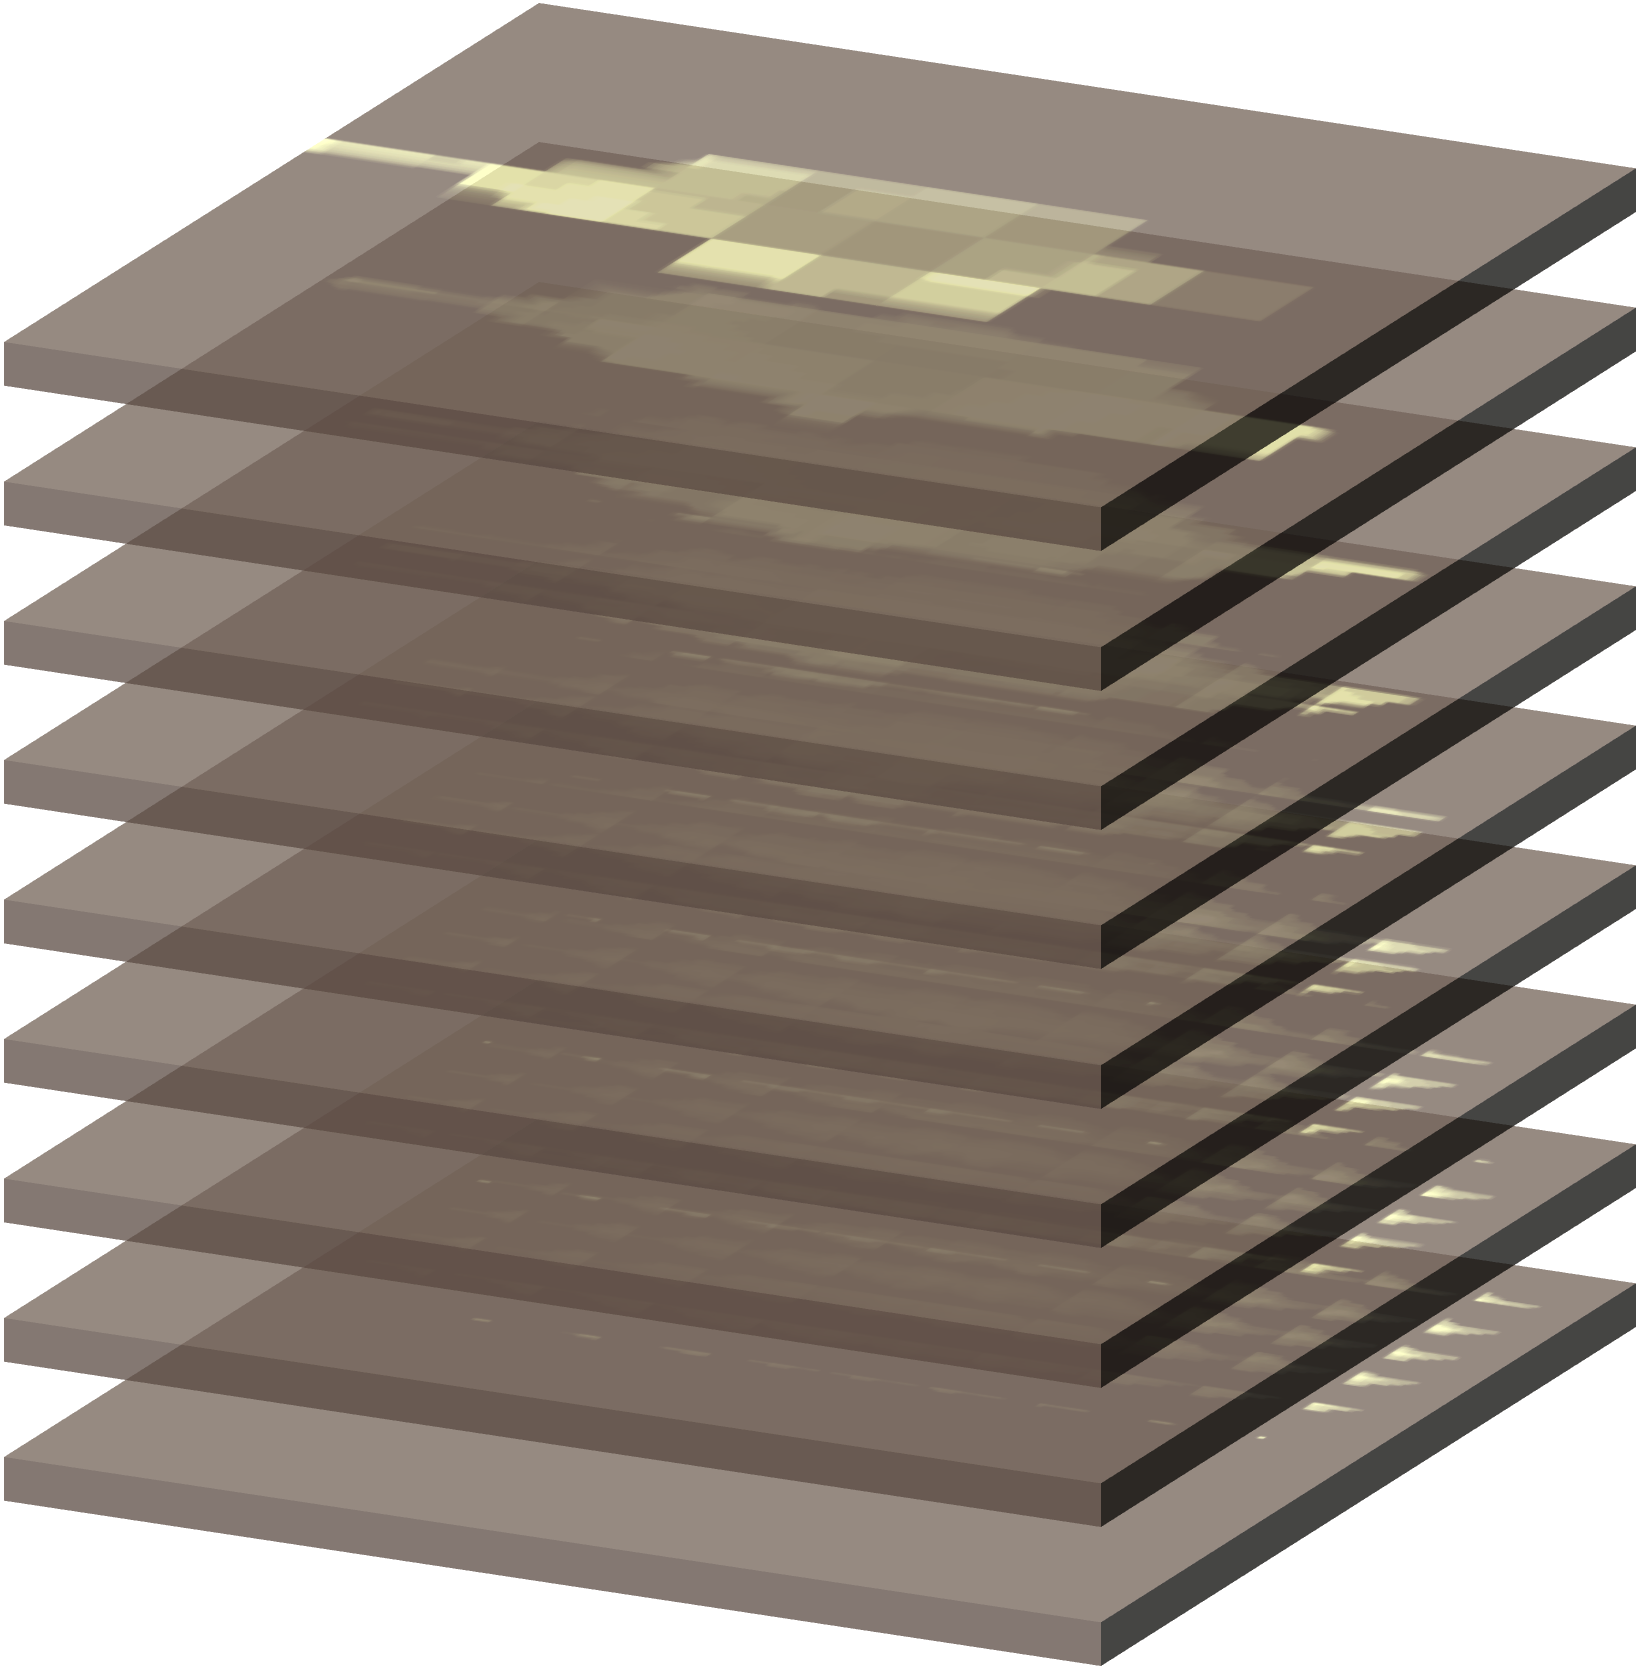
\includegraphics[width=0.675\linewidth]{figures/ivae/muon/muon-observations-stacked.png}};

            \node[inner sep=0, right=3cm of obs, label={[above, font=\LARGE, xshift=-5mm]:true state $s$}] (state) {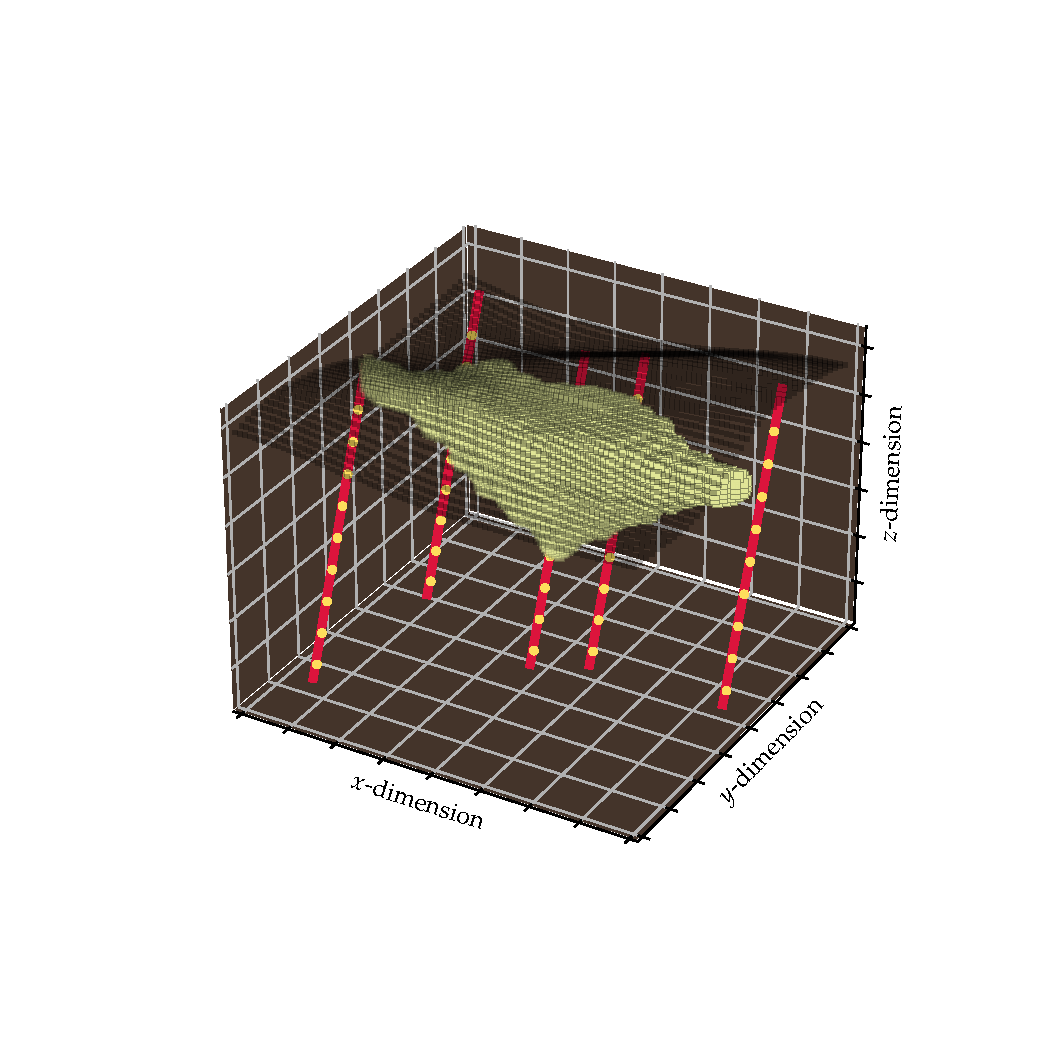
\includegraphics[trim=100 90 60 100, clip]{figures/ivae/muon/3d-intrusion.pdf}};
 
            \node[inner sep=0] (legend) at ($(state.south east)+(-64mm,25mm)$) {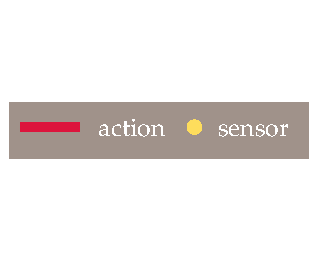
\includegraphics[trim=0 0 0 0, clip]{figures/ivae/muon/3d-intrusion-legend.pdf}};
 
            \draw[->, thick] (obs) -- (state) node[above, midway, font=\Large] {inversion} node[below, midway, font=\Large] {$f^{-1}$};
        \end{tikzpicture}
    }
    \caption{Example 3D inversion using muon tomography data ($5$ actions, $9$ sensors each).}
    \label{fig:muon_intrusion_diagram}
\end{figure}

To develop a likelihood-free posterior sampling method for POMDP planning, we extend the \textit{conditional variational autoencoder} (CVAE) model \cite{sohn2015learning} and fine-tune to maximize mutual information across observations from the same state---thereby, allowing latent observation trajectories to be more consistent across time.
As with the CVAE, we train using states and partial observations but only require partial observations during inference for conditioning.


\subsection{Related Work}
This work can be viewed as learning a generative model that samples states that are reconstructed from partial observations.
For our work, we consider the states and observations to be images (partial images for observations); therefore, generative modeling research from the computer vision community can be directly applicable.

\paragraph{Probabilistic generative models.}
A variety of deep generative models have been proposed to learn complex data distributions and enable conditional sampling. Variational autoencoders (VAEs) \cite{kingma2013vae,rezende2014stochastic} frame the density estimation problem as approximate Bayesian inference and train an encoder-decoder architecture to maximize a variational lower bound on the data likelihood $p_\theta(s)$.
Conditional VAEs (CVAEs) extend this framework by incorporating conditional information (e.g., labels or partial observations) into both the encoder and decoder, enabling conditional generation via $p_\theta(s \mid \mathbf{o})$ \cite{sohn2015learning}.
We detail the VAE and CVAE generative model architectures in the following section.
Other approaches, such as generative adversarial networks (GANs) \cite{goodfellow2014generative}, formulate generation as a two-player minimax game between a generator and a discriminator, achieving high-fidelity samples but often suffering from instability and mode collapse \cite{metz2016unrolled}.
\textcite{mirza2014conditional} introduced conditional GANs (CGANs), which extend traditional GANs by guiding the generator-discriminator framework with conditioning variables.
Beyond VAEs and GANs, normalizing flows \cite{rezende2015variational} provide exact likelihood evaluation through a sequence of invertible transformations, while more recent score-based and diffusion models \cite{ho2020denoising,song2021score} demonstrate state-of-the-art sample quality by learning to reverse a data corruption process.
In the context of online planning, diffusion models may be prohibitively expensive, as a single state sample typically requires on the order of $10^3$ sequential neural network forward passes \cite{ho2020denoising,nichol2021improved,janner2022planning}.
Our work extends these deep conditional generative models specifically for inversion problems, where we ensure both reconstruction consistency and guide fine-tuning using mutual information to generate state samples given partial observations.
For a more detailed overview of different classes of generative models, see \textcite{cao2023comprehensive}.

\paragraph{Deterministic inversion methods.}
In geological research, inversion problems \cite{tarantola1987inverse} can be viewed as computing a function that reconstructs some hidden state of the world given some (noisy) observation, generally geophysical measurements such as gravity data \cite{huang2021deep}, active seismic imaging \cite{deng2022openfwi}, or density data from passive muon tomography \cite{lechmann2021muon}.
Deep learning models have been applied to geological inversion problems primarily through the use of deterministic convolutional neural networks (CNNs) \cite{puzyrev2019deep,hu2021inversion}.
In these settings, a neural network is trained to perform regression $s = f_\theta(\mathbf{o}_{1:T})$ given full observations.
In our work, we consider the case where the observations are only partially observed (e.g., partial borehole data or partial geophysical data), yet a full state is sampled from the model.
Other approaches, such as linear and nonlinear least-squares methods as well as regularization techniques, have been explored in the deterministic inversion literature \cite{menke1989geophysical,tikhonov1963solution,constable1987occam,parker1994geophysical}.
Principal component analysis (PCA) and kernel PCA have also been used as dimensionality reduction techniques for deterministic history matching \cite{reynolds1996reparameterization,esmaeili2020kernel}.
\textcite{tarantola2005inverse} and, more recently, \textcite{zhdanov2015geophysical} provide comprehensive reviews of existing deterministic inversion methods applied to geological problems.


\paragraph{Probabilistic inversion methods.}
To quantify the uncertainty in the hidden state, probabilistic inversion methods---similar to probabilistic generative models---have been extensively studied.
\textcite{mcaliley2024stochastic} use a straightforward implementation of a conditional VAE to invert geophysical data and sample from a unit Gaussian $z \sim \mathcal{N}(\mathbf{0}, \mathbf{I})$ during inference, as is standard in most CVAE applications.
Their approach omits any observation encoder as the observations are vectors of synthetic gravity.
In our work, we are interested in high-dimensional observations where a separate observation encoder is useful for dimensionality reduction and we learn latent Gaussian parameters $\mu_\mathbf{o}$ and $\log \sigma^2_\mathbf{o}$ directly.
\textcite{chung2024paired} proposed a paired autoencoder approach but rely on an initial guess of the true state during inference and learn an observation decoder alongside a state decoder, which may not be necessary for strictly observation-to-state intrusion, as we show in our experiments.
Other sampling techniques have also been studied such as Markov chain Monte Carlo (MCMC) \cite{metropolis1953equation,hastings1970monte,mosegaard1995monte}.
\textcite{laloy2017inversion} condition based on expensive MCMC steps and suggest long runs to generate larger Markov chains for full exploration of the posterior, which may be expensive for planning.
In a recent survey on neural network-based geological inversion, \textcite{li2023comprehensive} identify a need for efficient probabilistic inversion methods.


\section{Background}\label{sec:vae_background}
This section provides background on probabilistic generative models that serve as the basis for our work.
Specifically, we review the variational autoencoder and its conditional variant.

\begin{figure}[t]
    \centering
    \resizebox{0.8\linewidth}{!}{
        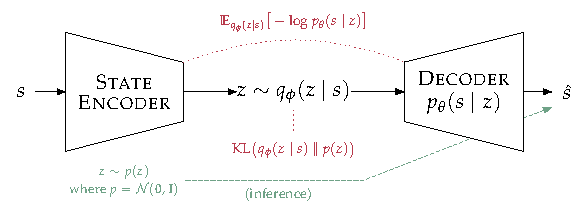
\includegraphics[trim=0 5 0 5, clip]{diagrams/ivae/vae.pdf}
    }
    \caption{The variational autoencoder (VAE) architecture and loss.}
    \label{fig:vae}
\end{figure}

\subsection{Variational Autoencoder}

\textcite{kingma2013vae} introduced the \textit{variational autoencoder} (VAE), a probabilistic model used for approximate inference with continuous latent variables.
The VAE is designed to approximate the generative model $p(s)$ by assuming the variables $s$ are sampled following some hidden process.
This process consists of first sampling a hidden random variable $z \sim p_\theta(z)$, then generating a state sample using the latent $z$ as a condition $s \sim p_\theta(s \mid z)$. 
This assumes both the prior $p_\theta(z)$ and likelihood $p_\theta(s \mid z)$ come from some parametric family of distributions \cite{kingma2013vae}.
To approximate the intractable true posterior density of $p_\theta(z \mid s) = p_\theta(s \mid z)p_\theta(z) / p_\theta(s)$, a probabilistic \textit{encoder} model $q_\phi(z \mid s)$ is used (also called the \textit{recognition model}).
Similarly, $p_\theta(s \mid z)$ is referred to as the probabilistic \textit{decoder} (or the \textit{generation model}).

The objective when training a VAE is to maximize the marginal likelihood $p(s^{(i)})$.
\textcite{kingma2013vae} show that the objective can be approximated by the \textit{variational lower bound} (ELBO):
\begin{equation}
    \log p_\theta\big(s^{(i)}\big) \ge \mathbb{E}_{q_\phi(z \mid s)} \big[-\log q_\phi(z \mid s) + \log p_\theta(s, z)\big]
\end{equation}
where $\theta$ and $\phi$ are the parameters of the generation model and recognition model, respectively.
Because the objective is to maximize the marginal log-likelihood, we can minimize the following loss using standard gradient-based optimization methods \cite{kingma2014adam}:
\begin{align}
    \mathcal{L}_\text{VAE}(s; \phi, \theta) = \displaystyle \mathbb{E}_{q_\phi(z \mid s)} \big[ -\log p_\theta(s \mid z) \big] + \operatorname{KL}\!\big(q_\phi(z \mid s) \,\Vert\, p(z)\big)
\end{align}
\Cref{fig:vae} visualizes the probabilistic encoder-decoder model of the variational autoencoder.

\begin{figure}[t]
    \centering
    \resizebox{0.8\linewidth}{!}{
        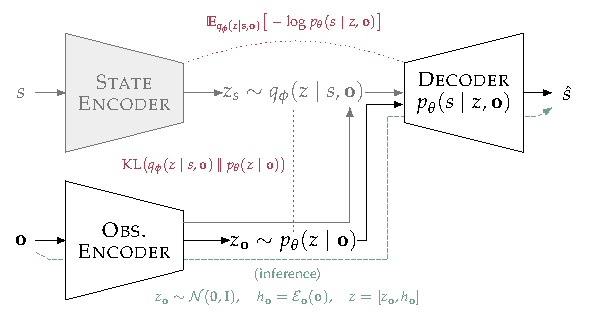
\includegraphics{diagrams/ivae/cvae.pdf}
    }
    \caption{The conditional variational autoencoder (CVAE) architecture and loss.}
    \label{fig:cvae}
\end{figure}

\subsection{Conditional Variational Autoencoder}
As a natural extension to VAEs, \textcite{sohn2015learning} introduced the \textit{conditional variational autoencoder} (CVAE), illustrating the model architecture in \cref{fig:cvae}.
The CVAE is comprised of a recognition (state encoder) model $q_\phi(z \mid s, \mathbf{o})$, the conditional prior (observation encoder) model $p_\theta(z \mid \mathbf{o})$, and the generation (decoder) model $p_\theta(s \mid z, \mathbf{o})$.
The objective of the CVAE model is to maximize $p(s \mid \mathbf{o})$, i.e., the conditional likelihood of the data $s$ given a condition $\mathbf{o}$ (a partial observation in our case).
\textcite{sohn2015learning} derive a conditional extension of the variational lower bound as:
\begin{align}
    \log p_\theta(s \mid \mathbf{o}) &\ge \mathbb{E}_{q_\phi(z \mid s, \mathbf{o})}\big[-\log q_\phi(z \mid s, \mathbf{o}) + \log p_\theta(s, z \mid \mathbf{o})\big] \\
    &= \mathbb{E}_{q_\phi(z \mid s, \mathbf{o})}\big[-\log q_\phi(z \mid s, \mathbf{o}) + \log p_\theta(z \mid \mathbf{o})\big] + \mathbb{E}_{q_\phi(z \mid s, \mathbf{o})}\big[\log p_\theta(s \mid z, \mathbf{o})\big] \nonumber
\end{align}
Minimizing the following loss approximates maximizing the conditional log-likelihood:
\begin{align}
    \mathcal{L}_\text{CVAE}(s, \mathbf{o}; \phi, \theta) = \displaystyle \mathbb{E}_{q_\phi(z \mid s, \mathbf{o})} \big[ -\log p_\theta(s \mid z, \mathbf{o}) \big] + \operatorname{KL}\!\big(q_\phi(z \mid s, \mathbf{o}) \,\Vert\, p_\theta(z \mid \mathbf{o})\big)
\end{align}
\textcite{sohn2015learning} input both the observation $\mathbf{o}$ and an initial guess of the state $\hat{s}$ from a separate CNN for better structured output predictions \cite{pinheiro2014recurrent,sohn2014improved}. In our experiments, we omit this step to focus on the core model differences, yet this recurrent connection could easily be implemented for more refined generative predictions.

\begin{figure}[t]
    \centering
    \resizebox{0.9\linewidth}{!}{
        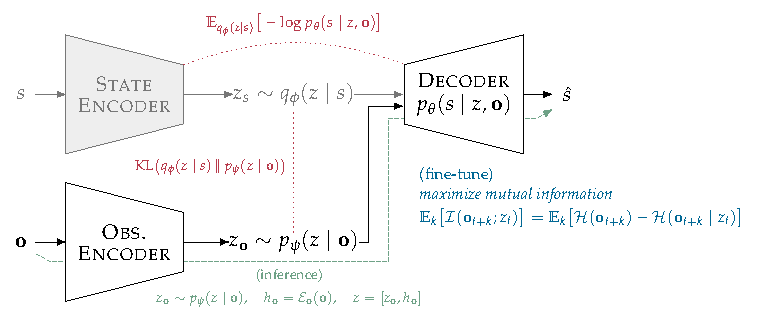
\includegraphics{diagrams/ivae/ivae.pdf}
    }
    \caption{The inversion variational autoencoder ($\mathcal{I}$-VAE) architecture and loss.}
    \label{fig:ivae}
\end{figure}


\section{Inversion Variational Autoencoder}
Using conditional generative models in sequential decision making problems can act as a way to sample (hidden) states conditioning on the set of observations up to time $t$.
Knowing that the generative model will be used during sequential planning means we will have sets of observations from different time steps that each correspond to some true state.
Therefore, we extend the CVAE model in three ways: (1) simplify the network design so that the recognition model depends only on the state, (2) directly learn the parameters $\psi$ of the conditional prior model $p_\psi(z \mid \mathbf{o})$ instead of a unit Gaussian \cite{sohn2015learning,walker2016uncertain,babaeizadeh2018stochastic}, and (3) fine-tune the model to maximize mutual information \cite{oord2018representation} across observation trajectories, ensuring trajectories from the same state are closer together in the latent space and trajectories from differing states are further apart.
In the EMDP setting, our belief update results in an inversion problem.
Therefore, we propose the \textit{inversion variational autoencoder} ($\mathcal{I}$-VAE) to address these challenges, illustrated in \cref{fig:ivae}.

The following $\mathcal{I}$-VAE loss function differs from the CVAE loss simply in the proposal $q_\phi$.
The CVAE proposal conditions on both the state $s$ and observation $\mathbf{o}$, namely $q_\phi(z \mid s, \mathbf{o})$, while the $\mathcal{I}$-VAE proposal removes the dependence on the observation, namely $q_\phi(z \mid s)$.
The difference lies in applying conditional independence $z \,\bot\, \mathbf{o} \mid s$ which implies that once we know the state $s$, the observation $\mathbf{o}$ provides no additional information.
This simplifies the network architecture without compromising performance (see analysis in \cref{sec:ivae_experiments}).

\subsection{$\mathcal{I}$-VAE Pretraining Objective}

The following pretraining loss function is derived in a similar manner to the CVAE loss, using the conditional variational lower bound (ELBO).
To derive the $\mathcal{I}$-VAE loss function, we begin with the objective to approximate the following conditional distribution:
\begin{equation}
    p(s \mid \mathbf{o}) = \int p(s, z \mid \mathbf{o}) \diff z \label{eq:ivae_objective}
\end{equation}
Similar to the variational lower bound derivation for CVAEs \cite{sohn2015learning}, we get the following:
\begin{align}
    \log p(s \mid \mathbf{o}) &= \log \int p(s, z \mid \mathbf{o}) \diff z && \\
    &= \log \int p(s \mid z, \mathbf{o}) p(z \mid \mathbf{o}) \diff z \label{eq:ivae_cr} \\
    &= \log \int q_\phi(z \mid s) \frac{p(s \mid z, \mathbf{o})p(z \mid \mathbf{o})}{q_\phi(z \mid s)} \diff z \label{eq:ivae_introduce_q} \\
    &\approx \log \int q_\phi(z \mid s) \frac{p_\theta(s \mid z, \mathbf{o})p_\psi(z \mid \mathbf{o})}{q_\phi(z \mid s)} \diff z \label{eq:ivae_introduce_qp} \\
    &\ge \int q_\phi(z \mid s) \log\left( \frac{p_\theta(s \mid z, \mathbf{o})p_\psi(z \mid \mathbf{o})}{q_\phi(z \mid s)} \right) \diff z \label{eq:ivae_jensens} \\
    &= \mathbb{E}_{q_\phi(z \mid s)} \left[ \log\left( p_\theta(s \mid z, \mathbf{o}) \frac{p_\psi(z \mid \mathbf{o})}{q_\phi(z \mid s)} \right) \right] \label{eq:ivae_expectation_def} \\
    &= \mathbb{E}_{q_\phi(z \mid s)} \left[ \log p_\theta(s \mid z, \mathbf{o}) \right] + \mathbb{E}_{q_\phi(z \mid s)} \left[ \log\left( \frac{p_\psi(z \mid \mathbf{o})}{q_\phi(z \mid s)} \right) \right] \label{eq:ivae_rules} \\
    &= \mathbb{E}_{q_\phi(z \mid s)}[\log p_\theta(s \mid z, \mathbf{o})] - \operatorname{KL}\big(q_\phi(z \mid s) \,\Vert\, p_\psi(z \mid \mathbf{o})\big) \label{eq:ivae_kl}
\end{align}
where \cref{eq:ivae_cr} applies the chain rule,
\cref{eq:ivae_introduce_q} introduces the proposal distribution $q_\phi(z \mid s) / q_\phi(z \mid s)$, \cref{eq:ivae_introduce_qp} introduces the learnable approximations $p_\theta(s \mid z, \mathbf{o}) \approx p(s \mid z, \mathbf{o})$ and $p_\psi(z \mid \mathbf{o}) \approx p(z \mid \mathbf{o})$, \cref{eq:ivae_jensens} applies Jensen's inequality, \cref{eq:ivae_expectation_def,eq:ivae_rules} apply expectation and logarithmic rules, and finally \cref{eq:ivae_kl} applies the definition of KL-divergence.


\begin{figure}[t]
    \centering
    \resizebox{0.9\linewidth}{!}{
        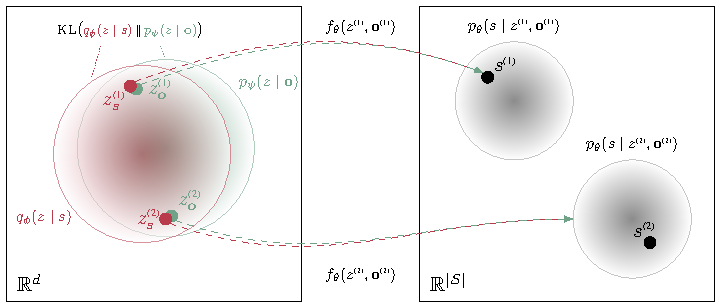
\includegraphics{diagrams/ivae/ivae_mapping.pdf}
    }
    \caption{Latent space matching of $z_s$ and $z_\mathbf{o}$ and mapping to $p_\theta(s \mid z, \mathbf{o})$ for the $\mathcal{I}$-VAE.}
    \label{fig:mapping}
\end{figure}


To train surrogates to approximate this distribution, we want to minimize the negative log-likelihood to get the $\mathcal{I}$-VAE (pretraining) loss function:
\begin{align}
    \mathcal{L}_{\mathcal{I}\text{-VAE}}(s, \mathbf{o}; \phi, \theta, \psi) = \displaystyle \underbrace{\mathbb{E}_{q_\phi(z \mid s)} \big[ -\log p_\theta(s \mid z, \mathbf{o}) \big]}_{\substack{\text{Reconstruction loss}}} + \underbrace{\operatorname{KL}\!\big(q_\phi(z \mid s) \,\Vert\, p_\psi(z \mid \mathbf o)\big)}_{\substack{\text{KL-divergence}\\\text{(match latent distributions)}}} \label{eq:ivae_loss}
\end{align}
Intuitively, the $\mathcal{I}$-VAE loss function attempts to reconstruct the state $s$ from the latent variable $z$ and match the latent conditional distributions $q_\phi(z \mid s)$ and $p_\psi(z \mid \mathbf{o})$ by minimizing their KL-divergence.
\Cref{fig:mapping} illustrates this distribution matching.
The KL-divergence term acts both as a regularizer\footnote{The KL-divergence stops $q_\phi(z \mid s)$ from mode-collapsing or becoming arbitrarily tight around each training sample $s$, and it prevents $p_\psi(z \mid \mathbf{o})$ from ignoring the observation $\mathbf{o}$ or becoming too broad.} \cite{kingma2013vae} and as a way to learn a latent distribution that relies solely on the observations $\mathbf{o}$ during runtime inference.
By penalizing their divergence, this forces both distributions to share some consistent latent structure, thus, forcing the latent distribution with partial information $\mathbf{o}$ to be close to the latent distribution with full information $s$.
The CVAE model also only requires the observation during inference, but traditionally \cite{sohn2015learning,walker2016uncertain,babaeizadeh2018stochastic} samples $z_\mathbf{o}$ from a unit Gaussian distribution and concatenates the encoded observation $z_\mathbf{o}$ to get $z = [z_\mathbf{o}, h_\mathbf{o}]$, where $h_\mathbf{o} = \mathcal{E}_\mathbf{o}(\mathbf{o})$ is the encoded observation and $z$ is passed to the decoder.
The $\mathcal{I}$-VAE model explicitly learns an approximate conditional model $p_\psi(z \mid \mathbf{o})$, which uses the observation directly to shape where in the latent space to sample from.
This results in matching the inference-time behavior with the training-time behavior.

Our work is related to the \textit{variational autoencoder with arbitrary conditioning} (VAEAC) \cite{ivanov2019variational}, but their model assumes the observed data is simply a mask of the hidden (full) data.
This is true for pixel observations from images (e.g., MNIST \cite{lecun1998gradient}, shown in \cref{fig:mapping_3d}), but breaks down in cases where the observations are over a different domain (e.g., muon tomography observations).
Our model does not make this assumption about the observations, and we show that it can work in both cases in the analysis \cref{sec:ivae_experiments}.

\paragraph{Latent space mapping and runtime inference.}
Illustrated in \cref{fig:mapping_3d}, the goal during pretraining is to map both the latent-state variable $z_s$ and latent-observation variable $z_\mathbf{o}$ to a lower-dimensional representation in $\mathbb{R}^d$.
Using the KL-divergence from \cref{eq:ivae_loss}, we expect these latent variables to map to a similar area in the lower $d$-dimensional space.
During runtime inference, the reduced-dimension latent $z_\mathbf{o}$ is used to sample states from $p_\theta(s \mid z, \mathbf{o})$ consistent with the observations.
\Cref{fig:mapping_3d} shows an example using masked $4\times4$ pixel observations for the MNIST dataset, where at time $t=30$ the total pixel coverage given by the observations is about $15\%$.
A set of state samples $\mathbf{s}$ can be directly used to represent samples from an updated belief in EMDP planning, and we show an example of what the mean belief may look like when sampling $100$ states efficiently in a single batched forward pass of the $\mathcal{I}$-VAE model.


\begin{figure}[t]
    \centering
    \resizebox{0.9\linewidth}{!}{
        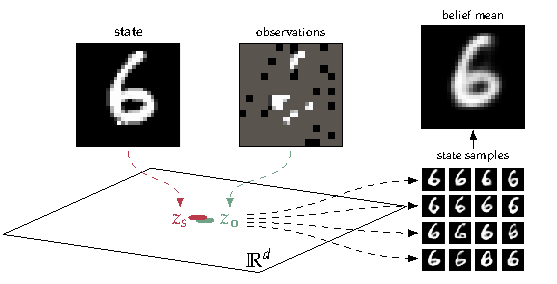
\includegraphics{diagrams/ivae/ivae_mapping_mnist.pdf}
    }
    \caption{Latent space mapping of $z_{o_{1:t}}$ ($t=30$) to $m=100$ state samples from $p_\theta(s \mid z, \mathbf{o})$.}
    \label{fig:mapping_3d}
\end{figure}


\paragraph{KL-divergence derivation.}
In practice, the latent distributions over $z$ are modeled as multivariate Gaussian distributions.
Given the probability density function of a multivariate Gaussian with diagonal covariance:
\begin{equation}
    \mathcal{N}\Big(z; \vec{\mu}, \operatorname{diag}\big(\vec{\sigma}^2\big)\Big) = \prod_{i=1}^{|z|} \frac{1}{\sqrt{2\pi\sigma_i^2}} \exp \left( - \frac{(z_i - \mu_i)^2}{2\sigma_i^2} \right)
\end{equation}
we analytically derive the KL-divergence between the latent state distribution $q_\phi(z \mid s)$ and the latent observation distribution $p_\psi(z \mid \mathbf{o})$ (where $(\vec{\mu}_s, \vec{\sigma}_s)$ and $(\vec{\mu}_\mathbf{o}, \vec{\sigma}_\mathbf{o})$ are the parameters of their respective distributions) as:
\begin{align}
    \operatorname{KL}\big(q_\phi(z \mid& s) \, \Vert \, p_\psi(z \mid \mathbf{o})\big) \\
    &= \int q_\phi(z \mid s) \log \!\left( \frac{q_\phi(z \mid s)}{p_\psi(z \mid \mathbf{o})} \right) \rm{d}z \\
    &= \int q_\phi(z \mid s) \log \!\left( \prod_{i=1}^{|z|} \frac{\big(2\pi\sigma_{s,i}^2\big)^{-1/2}\exp\big(-(z_i - \mu_{s,i})^2 / (2\sigma_{s,i}^2) \big)}{\big(2\pi\sigma_{\mathbf{o},i}^2\big)^{-1/2}\exp\big(-(z_i - \mu_{\mathbf{o},i})^2 / (2\sigma_{\mathbf{o},i}^2) \big)} \right) \rm{d}z \\
    &= \int q_\phi(z \mid s) \sum_{i=1}^{|z|} \left( \log\!\left(\frac{\sigma_{\mathbf{o},i}}{\sigma_{s,i}} \right) - \frac{(z_i - \mu_{\mathbf{o},i})^2}{2\sigma_{\mathbf{o},i}^2} + \frac{(z_i - \mu_{s,i})^2}{2\sigma_{s,i}^2} \right) \rm{d}z \\
    &= \sum_{i=1}^{|z|} \int q_\phi(z_i \mid s) \left( \log\!\left(\frac{\sigma_{\mathbf{o},i}}{\sigma_{s,i}} \right) - \frac{(z_i - \mu_{\mathbf{o},i})^2}{2\sigma_{\mathbf{o},i}^2} + \frac{(z_i - \mu_{s,i})^2}{2\sigma_{s,i}^2} \right) \rm{d}z \\
    &= \sum_{i=1}^{|z|} \left( \frac{1}{2} \Big( \log \sigma_{\mathbf{o},i}^2 - \log \sigma_{s,i}^2 \Big) - \frac{1}{2} + \frac{1}{2\sigma_{\mathbf{o},i}^2} \Big(\sigma_{s,i}^2 + (\mu_{s,i} - \mu_{\mathbf{o},i})^2 \Big) \right) \\
    &= \frac{1}{2} \sum_{i=1}^{|z|} \left( \log \sigma_{\mathbf{o},i}^2 - \log \sigma_{s,i}^2 + \frac{\sigma_{s,i}^2 + (\mu_{s,i} - \mu_{\mathbf{o},i})^2}{\sigma_{\mathbf{o},i}^2} - 1 \right)
\end{align}
More complex latent distributions could instead be used and have been extensively studied in the literature, such as Gaussian mixture models \cite{dilokthanakul2016deep,tomczak2018vae}, the Gumbel-Softmax distribution for categorical latents \cite{jang2017categorical}, normalizing flows \cite{rezende2015variational}, inverse autoregressive flows \cite{kingma2016improved}, and diffusion models \cite{kingma2021variational}.


\subsection{Fine-Tuning to Maximize Trajectory-Based Mutual Information}
Not only are we interested in modeling $p(s \mid \mathbf{o})$ from \cref{eq:ivae_objective}, we are also interested in the setting where sequences of observations will be passed to the model over time.
Thus, a secondary objective is to maximize mutual information between observation sequences (i.e., observation trajectories), to better align the latent space across observations correlated to the same state.
Therefore, we fine-tune the pretrained $\mathcal{I}$-VAE model with a \textit{trajectory contrastive loss} (TCL) \cite{oord2018representation,halawa2022action,zheng2023taco}.
The key idea is that once we have a performant generative model with trained encoders and decoder, we can further align the latent space given observation trajectories from a dataset $\big(s,\mathbf{o}_{1:T}\big) \in \mathcal{D}_\text{traj}$ of states and their observations over time.

The trajectory contrastive loss is a form of the InfoNCE loss \cite{oord2018representation}, where we want to maximize mutual information $\mathcal{I}$ between a window of $k \in [1,\ldots,K]$ observations and the observation-inferred latent variables $z_t$. Namely, we want to maximize the expectation of $\mathcal{I}(\mathbf{o}_{t+k}; z_t)$ over the $K$-length window, or minimize the negation:
\begin{align}
    \mathcal{L}_\text{TCL}(\mathbf{o}_{1:T}; \omega, K) &= -\mathbb{E}_k[\mathcal{I}(\mathbf{o}_{t+k}; z_t)] \label{eq:tcl} \\
        &= -\mathbb{E}_k[\mathcal{H}(\mathbf{o}_{t+k}) - \mathcal{H}(\mathbf{o}_{t+k} \mid z_t)] \quad \text{for} \quad 1 \le k \le K \\
        &= -\mathbb{E}_k \left[ \mathbb{E}_{z_t} \left[ \log \frac{p(\mathbf{o}_{t+k} \mid z_t)}{p(\mathbf{o}_{t+k})} \right] \right] \\
        &\ge -\mathbb{E}_k \left[ \mathbb{E}_{\tilde{z}} \left[ \log \frac{f(\mathbf{o}^+, \tilde{z})}{\sum_{\mathbf{o} \in \Omega^-} f(\mathbf{o}, \tilde{z})} \right] \right]
\end{align}
where $\mathcal{I}(a,b)$ represents the mutual information between $a$ and $b$, entropy is denoted by $\mathcal{H}$, the space $\Omega^- = \{\Omega \setminus \mathbf{o}^+\}$ is over all observation sequences excluding the positive observation $\mathbf{o}^+$, the latent $\tilde{z} = \Pi_\omega(\mu_{\mathbf{o}_t})$ is the output of a projection network parameterized by $\omega$, and the function $f$ measures the similarity between the observation $\mathbf{o}_t$ and projected latent variable $\tilde{z}$, following \textcite{oord2018representation}:
\begin{align}
    f(\mathbf{o}_t, \tilde{z}) = \exp \left(\frac{\tilde{z}^\top h_t}{\Vert \tilde{z} \Vert \Vert h_t \Vert} / \tau \right) \quad \text{where} \quad h_t = \mathcal{E}_\mathbf{o}(\mathbf{o}_t)
\end{align}
where $\tau$ is a temperature parameter.
For a window of length $K$, by minimizing the loss $\mathcal{L}_\text{TCL}$, we maximize mutual information for observation trajectories from $\mathbf{o}_{t}$ to $\mathbf{o}_{t+K}$.
The idea is that we want to optimize the latent space so that observations that come from the same sequence are closer together, while observations from different sequences are further apart.
In addition to fine-tuning the mutual information, we also want to preserve reconstruction and generation.
Therefore, the fine-tuning $\mathcal{I}$-VAE loss function then becomes:
\begin{equation}
    \mathcal{L}(s, \mathbf{o}_{1:T}; \omega, \theta, \phi, \psi, K) = \alpha \mathcal{L}_\text{TCL}(\mathbf{o}_{1:T}; \omega, K) + \mathbb{E}_{t} \Big[\mathcal{L}_{\mathcal{I}\text{-VAE}}^{(t)}(s, \mathbf{o}_t; \theta, \phi, \psi)\Big]
\end{equation}
The TCL loss acts as a self-supervised consistency loss on the observation encoder, helping it produce a smooth, predictive latent path \cite{zheng2023taco}.
In practice, we train the projection network $\Pi_\omega$ to discriminate between observation trajectories.

\paragraph{Training and inference.}
The $\mathcal{I}$-VAE training procedure and forward pass are detailed in \cref{alg:ivae_training,alg:ivae_forward}.
During runtime inference, the input observation is encoded to get $h_\mathbf{o} = \mathcal{E}_\mathbf{o}(\mathbf{o})$, a latent-observation variable $z_\mathbf{o}$ is sampled from $p_\psi(z \mid \mathbf{o})$, and a sampled state is reconstructed from the decoder $p_\theta(s \mid z, \mathbf{o})$ using $z = [z_\mathbf{o}, h_\mathbf{o}]$.

\begin{figure}[b!]
    \begin{algorithm}[H]
    \caption{$\mathcal{I}$-VAE training procedure.}
    \label{alg:ivae_training}
    \begin{algorithmic}[1]
    \Require $\theta, \phi, \psi, \omega \leftarrow \text{initialize network parameters}$
    \Require $\alpha \leftarrow \text{trajectory contrastive loss weighting}$
    \Require $\tau \leftarrow \text{trajectory contrastive loss temperature}$
    \Require $T \leftarrow \text{observation horizon}$
    \For{$\text{epoch} \leftarrow 1 \textbf{ to } n_\text{pretrain}$}
        \State Sample $(s, \mathbf{o})$ from $\mathcal{D}_\text{partial}$
        \State Forward pass $(s, \mathbf{o})$ to get $(\hat{s}, \mu_s, \log \sigma^2_s,\mu_\mathbf{o},\log \sigma^2_\mathbf{o})$ calling \cref{alg:ivae_forward}
        \State Compute loss $\mathcal{L}_{\mathcal{I}\text{-VAE}}(s, \mathbf{o}; \theta, \phi, \psi)$ given $(\hat{s},\, \log \sigma^2_s,\, \mu_\mathbf{o},\, \log \sigma^2_\mathbf{o})$ with \cref{eq:ivae_loss}
        \State Train $\theta$, $\phi$, and $\psi$
    \EndFor
    \For{$\text{epoch} \leftarrow 1 \textbf{ to } n_\text{fine-tune}$}
        \State Sample $(s, \mathbf{o}_{1:T})$ from $\mathcal{D}_\text{traj}$
        \State Compute $\mu_s$ and $\log \sigma^2_s$ from state encoder $\mathcal{E}_s(s)$
        \For{$t \leftarrow 1 \textbf{ to } T$}
            \State Encode $h_{\mathbf{o}_t}$ from observation encoder $\mathcal{E}_\mathbf{o}(\mathbf{o}_t)$ using $\mathbf{o}_t \in \mathbf{o}_{1:T}$
            \State Compute $\mu_{\mathbf{o}_t}$ and $\log \sigma^2_{\mathbf{o}_t}$ from $p_\psi(z \mid \mathbf{o}_t)$ using observation encoding $h_{\mathbf{o}_t}$
            \State Project $\tilde{z} = \Pi_\omega(\mu_{\mathbf{o}_t})$
            \State Decode $\hat{s}_t$ from $p_\theta(s \mid \tilde{z}, \mathbf{o})$
            \State Compute $\mathcal{L}_t = \mathcal{L}_{\mathcal{I}\text{-VAE}}(s, \mathbf{o}_t; \theta, \phi, \psi)$ from \cref{eq:ivae_loss} using $\hat{s}_t$
        \EndFor
        \State Compute combined loss $\mathcal{L} = \alpha \mathcal{L}_\text{TCL}(\mathbf{o}_{1:T}; \omega, K) + \mathbb{E}_t[\mathcal{L}_t]$ using \cref{eq:tcl}
        \If{$\text{epoch} = 1$}
            \State Train projection network parameters $\omega$
        \Else
            \State Train $\omega$ and $\psi$ (optional: $\theta$ and $\phi$)
        \EndIf
    \EndFor
    \end{algorithmic}
\end{algorithm}

    \begin{algorithm}[H]
    \caption{$\mathcal{I}$-VAE forward pass.} 
    \label{alg:ivae_forward}
    \begin{algorithmic}[1]
    \Require $s, \mathbf{o}$ (state and observations)
    \State Compute $h_s$, $\mu_s$, and $\log \sigma^2_s$ from state encoder $h_s = \mathcal{E}_s(s)$ and $q_\phi(z \mid s)$
    \State Sample $z \sim q_\phi(z \mid s)$ using state encoding $h_s$
    \State Compute $h_\mathbf{o}$, $\mu_\mathbf{o}$, and $\log \sigma^2_\mathbf{o}$ from observation encoder $h_\mathbf{o} = \mathcal{E}_\mathbf{o}(\mathbf{o})$ and $p_\psi(z \mid \mathbf{o})$
    \State Decode $\hat{s}$ from $p_\theta(s \mid z, \mathbf{o})$ using $z$ and observation encoding $h_\mathbf{o}$
    \State \Return $(\hat{s}, \mu_s, \log \sigma^2_s, \mu_\mathbf{o}, \log \sigma^2_\mathbf{o})$
    \end{algorithmic}
\end{algorithm}

\end{figure}

\section{Experiments and Analysis}\label{sec:ivae_experiments}
We demonstrate the effectiveness of the $\mathcal{I}$-VAE on two sequential problems: partial MNIST observations \cite{lecun1998gradient} and a real-world muon tomography mineral exploration EMDP.
The model code,\footnote{\url{https://github.com/sisl/I-VAE}} written in PyTorch, and the muon observation EMDP code,\footnote{\url{https://github.com/sisl/MuonPOMDPs.jl}} written in Julia and Python, are open-sourced to extend to other problems and for reproducibility.
Details regarding hyperparameters and neural network architectures are included in the code.


\subsection{Pixel Observation Problem: MNIST}\label{sec:mnist_experiments}
Using the standard MNIST benchmark of hand-written digits, we are interested in measuring how well the model performs given partial observations.
We partition the image into $196$ chunks of $4 \times 4$ pixels each to act as a individual observations.
In this problem, the observations can be interpreted as a mask applied to the true (hidden) state.
Given random pixel observations over time, we refer to the ``unmasked'' observations as the observation coverage percentage (e.g., if $49$ out of $196$ chucks are uncovered, we have $25\%$ coverage).
We compare the $\mathcal{I}$-VAE model against a standard CVAE, a deterministic neural network (NN) baseline, and against the $\mathcal{I}$-VAE pretrained model (i.e., without fine-tuning with TCL).
All of the models are simple MLPs following parameters used by \textcite{sohn2015learning} for the original MNIST CVAE experiments.
To measure the quality of the models, we evaluate the conditional log-likelihood (CLL) across each observation coverage percentage \cite{sohn2015learning}:
\begin{equation}
    \log p_\theta(s \mid \mathbf{o}) \approx \log \left( \frac{1}{n} \sum_{i=1}^n p_\theta\big(s \mid z^{(i)}, \mathbf{o}\big) \right) \quad \text{where} \quad z^{(i)} \sim p_\psi(z \mid \mathbf{o}) \label{eq:cll}
\end{equation}
where $n$ is the size of the MNIST test dataset ($n = 10{,}000$).
The CLL metric is a standard way to evaluate the statistical performance of the models.


\Cref{tab:clls_mnist} shows the conditional log-likelihoods across the various models for different observation coverage percentages.
In the MNIST case, we observe that the $\mathcal{I}$-VAE without TCL performs just as well as the CVAE model.
The benefit of additional TCL fine-tuning is most evident in regimes with low observation coverage (e.g., no observations at $0\%$ and $25\%$ observation coverage).
Unsurprisingly, the neural network baseline performs the worst as it will deterministically infer a single state given the observations.


\begin{table*}[t!]
    \centering
    \begin{threeparttable}
        \begin{tabular}{@{}lrrrrr@{}}
            \toprule
            \multirow{2}{*}{Method} & \multicolumn{5}{c}{Conditional log-likelihood (CLL)} \\
            \cmidrule{2-6}
            & $0\%$ & $25\%$ & $50\%$ & $75\%$ & $100\%$ \\
            \midrule
            NN (baseline)  &  $-197.11$  &  $-93.44$  &  $-74.30$  &  $-66.83$  &  $-62.43$  \\
            CVAE  &  $-192.52$  &  $-86.89$  &  $-68.76$  &  $-63.19$  &  $-59.47$  \\
            $\mathcal{I}$-VAE (no TCL)  &  $-195.07$  &  $-87.15$  &  $-68.90$  &  $-62.97$  &  $-59.02$  \\
            $\mathcal{I}$-VAE  &  $\mathBF{-176.41}$  &  $\mathBF{-82.39}$  &  $\mathBF{-67.77}$  &  $\mathBF{-62.38}$  &  $\mathBF{-58.51}$  \\
            \bottomrule
        \end{tabular}
    \end{threeparttable}
    \caption{MNIST: CLLs given different observation coverage percentages.}
    \label{tab:clls_mnist}
\end{table*}


The better performance with less observation coverage is also evident in \cref{fig:clls_mnist}.
At observation coverages of around $30\%$ or less, the $\mathcal{I}$-VAE model has higher conditional log-likelihood than the CVAE.
Also evident in \cref{fig:clls_mnist} is that the $\mathcal{I}$-VAE model without TCL recovers CVAE performance---which is true in the MNIST example, but as we will see in the next section, both $\mathcal{I}$-VAE models outperform the CVAE when using an information-based heuristic planner, framing the sequential information gathering problem as an EMDP.


\begin{figure}[b!]
    \centering
    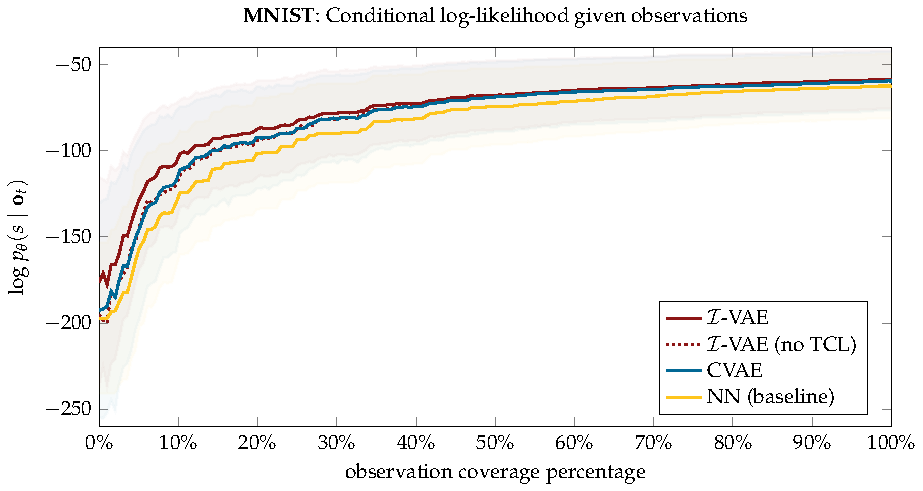
\includegraphics[width=0.815\linewidth]{figures/ivae/mnist/cll-mnist.pdf}
    \caption{Conditional log-likelihood over the MNIST test dataset ($\pm$ one stddev).}
    \label{fig:clls_mnist}
\end{figure}


\Cref{fig:mnist_unconditioned_priors} qualitatively illustrates how the $\mathcal{I}$-VAE can better reconstruct the data when conditioning on no observations (i.e., observation $\mathbf{o}$ is solely comprised of all $-1$ values).
In this unconditioned case, when the observation coverage is $0\%$, we can visually see that when sampling states with no observation information, the mean belief, shown in \cref{fig:mnist_data_prior,fig:mnist_ivae_prior,fig:mnist_cvae_prior}, matches closer to the MNIST test data prior.
We also visualize reconstructed samples, conditioned without any observation information in \cref{fig:mnist_data_samples,fig:mnist_ivae_samples,fig:mnist_cvae_samples}.

Finally, \cref{fig:mnist_ivae_images1,fig:mnist_ivae_images2} demonstrate additional qualitative analysis.
The figures show representative examples of taking random pixel observation actions from $0\%$ to $100\%$ coverage for the $\mathcal{I}$-VAE and CVAE.
We plot the mean belief over $1000$ samples and several generated state samples over time.
These results also indicate that the $\mathcal{I}$-VAE not only learns better and more diverse digit reconstructions, as evident by the more visually consistent predictions, but also converges to the correct state in fewer observations (about $10\%$ in \cref{fig:mnist_ivae_images1} and about $20\%$ in \cref{fig:mnist_ivae_images2}).
We also include the aggregate classification probabilities from a learned classification MLP\footnote{Following \textcite{imambi2021pytorch} for a simple MLP classification model from \url{https://github.com/pytorch/examples/blob/main/mnist/main.py}.} in the bottom row, further indicating the confidence in the prediction when aggregating over the $1000$ sampled states.
In the classification plots, the shaded bars represent the correct classification label.
In both models, when the observation coverage is high, the reconstruction recovers the true state.

\begin{figure}[t!]
    \captionsetup{font={small}}
    \centering
    \begin{subfigure}[t]{0.32\linewidth}
        \centering
        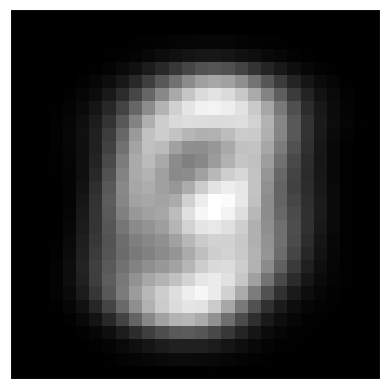
\includegraphics[width=0.9\linewidth]{figures/ivae/mnist/mnist-data-prior.png}
        \caption{MNIST test data prior.}
        \label{fig:mnist_data_prior}
    \end{subfigure}
    \hfill
    \begin{subfigure}[t]{0.32\linewidth}
        \centering
        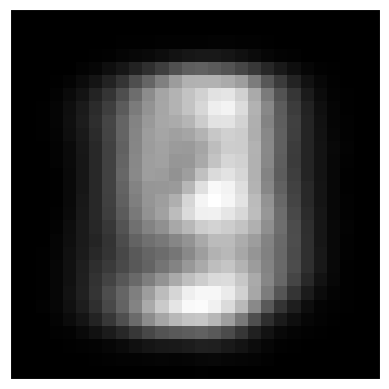
\includegraphics[width=0.9\linewidth]{figures/ivae/mnist/mnist-ivae-prior.png}
        \caption{$\mathcal{I}$-VAE unconditioned prior.}
        \label{fig:mnist_ivae_prior}
    \end{subfigure}
    \hfill
    \begin{subfigure}[t]{0.32\linewidth}
        \centering
        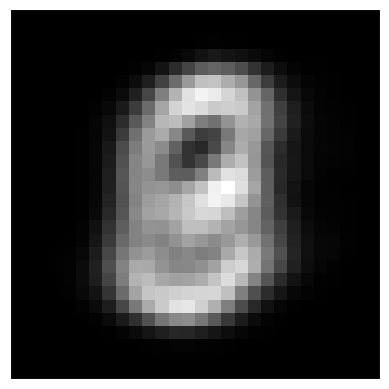
\includegraphics[width=0.9\linewidth]{figures/ivae/mnist/mnist-cvae-prior.png}
        \caption{CVAE unconditioned prior.}
        \label{fig:mnist_cvae_prior}
    \end{subfigure}

    \vspace*{5mm}

    \begin{subfigure}[t]{0.32\linewidth}
        \centering
        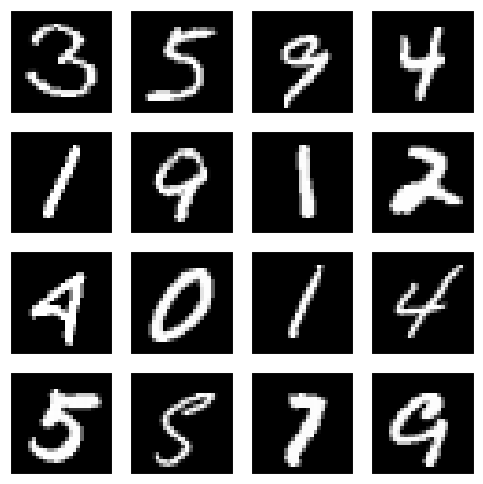
\includegraphics[width=0.9\linewidth]{figures/ivae/mnist/mnist-data-samples.png}
        \caption{Test data samples.}
        \label{fig:mnist_data_samples}
    \end{subfigure}
    \hfill
    \begin{subfigure}[t]{0.32\linewidth}
        \centering
        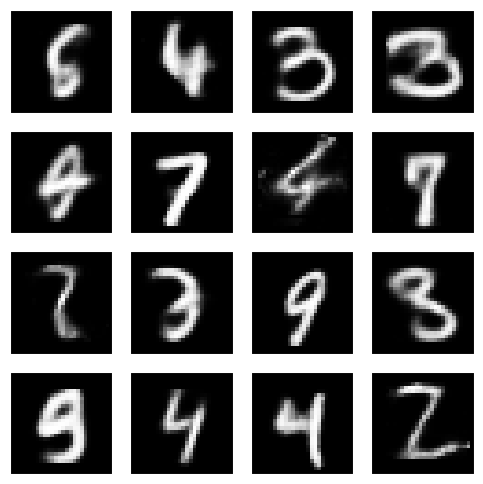
\includegraphics[width=0.9\linewidth]{figures/ivae/mnist/mnist-ivae-samples.png}
        \caption{$\mathcal{I}$-VAE unconditioned samples.}
        \label{fig:mnist_ivae_samples}
    \end{subfigure}
    \hfill
    \begin{subfigure}[t]{0.32\linewidth}
        \centering
        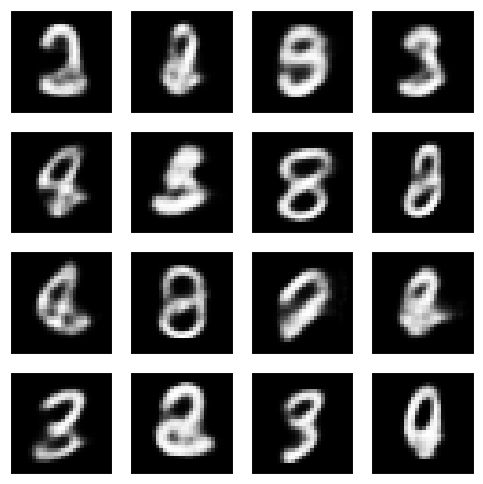
\includegraphics[width=0.9\linewidth]{figures/ivae/mnist/mnist-cvae-samples.png}
        \caption{CVAE unconditioned samples.}
        \label{fig:mnist_cvae_samples}
    \end{subfigure}
    \caption{Mean priors (i.e., no observations), sampling $m=1000$ for $\mathcal{I}$-VAE and CVAE.}
    \label{fig:mnist_unconditioned_priors}
\end{figure}


\begin{figure}[p]
    \hspace*{5.5mm}
    \resizebox{0.8\linewidth}{!}{
        \begin{tikzpicture}
            \node[inner sep=0] (img) at (0,0) {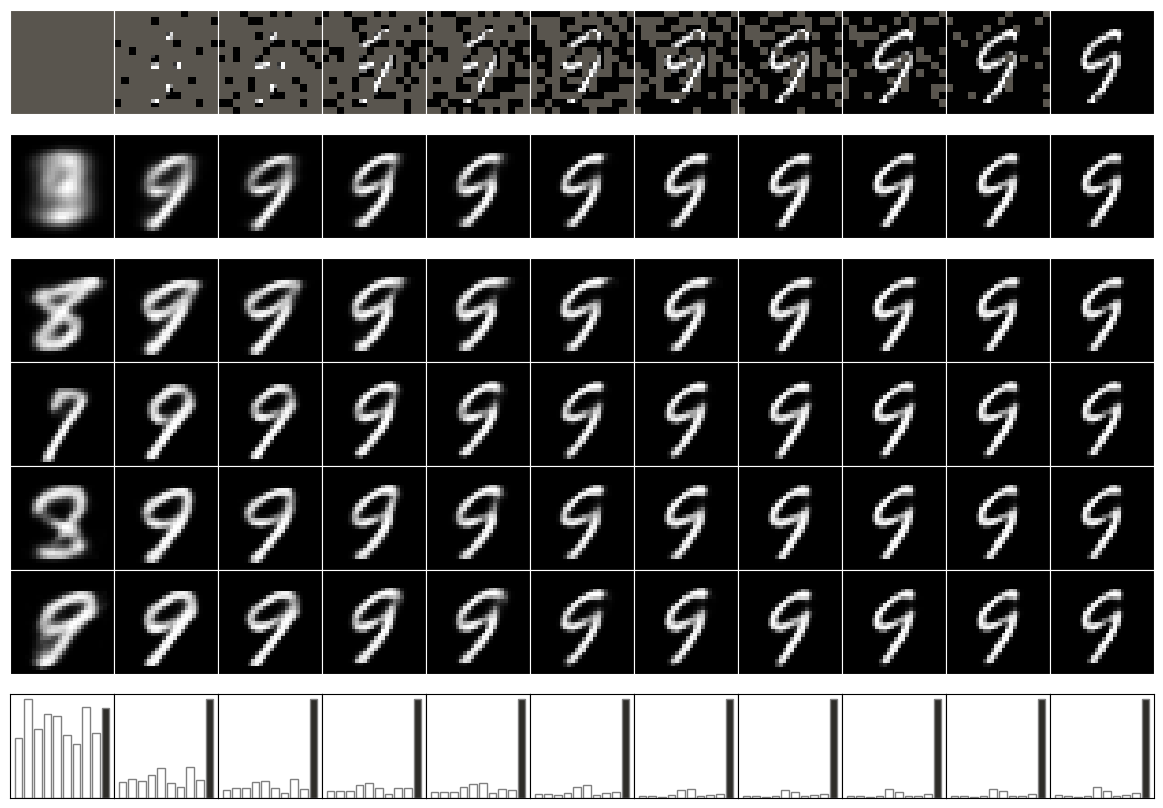
\includegraphics{figures/ivae/mnist/mnist-ivae-2.png}};
            
             \coordinate (left)  at ($(img.north west)!0.01!(img.north east)$);
            \coordinate (right) at ($(img.north west)!0.99!(img.north east)$);

            \foreach \i in {0,...,10} {
                \node[anchor=south] at ($(left)!{(\i + 0.5)/11}!(right)$) {{\fontsize{32}{36}\selectfont $\the\numexpr\i*10\relax\%$}};
            }

            \node[anchor=south] at ($(img.north)+(0,2.5)$) {{\fontsize{42}{48}\selectfont $\mathcal{I}$-VAE}};

            \node[anchor=east] at ($(img.north west)+(0,-2.2)$) {{\fontsize{32}{36}\selectfont observations}};
            \node[anchor=east] at ($(img.north west)+(0,-6.5)$) {{\fontsize{32}{36}\selectfont belief mean}};
            \node[anchor=east] at ($(img.north west)+(0,-10.8)$) {{\fontsize{32}{36}\selectfont state samples}};
            \node[anchor=east] at ($(img.south west)+(0,2.2)$) {{\fontsize{32}{36}\selectfont classification}};
            
        \end{tikzpicture}
    }
    
    \vspace*{15mm} % blank lines above and below are important

    \hspace*{5.5mm}
    \resizebox{0.8\linewidth}{!}{
        \begin{tikzpicture}
            \node[inner sep=0] (img) at (0,0) {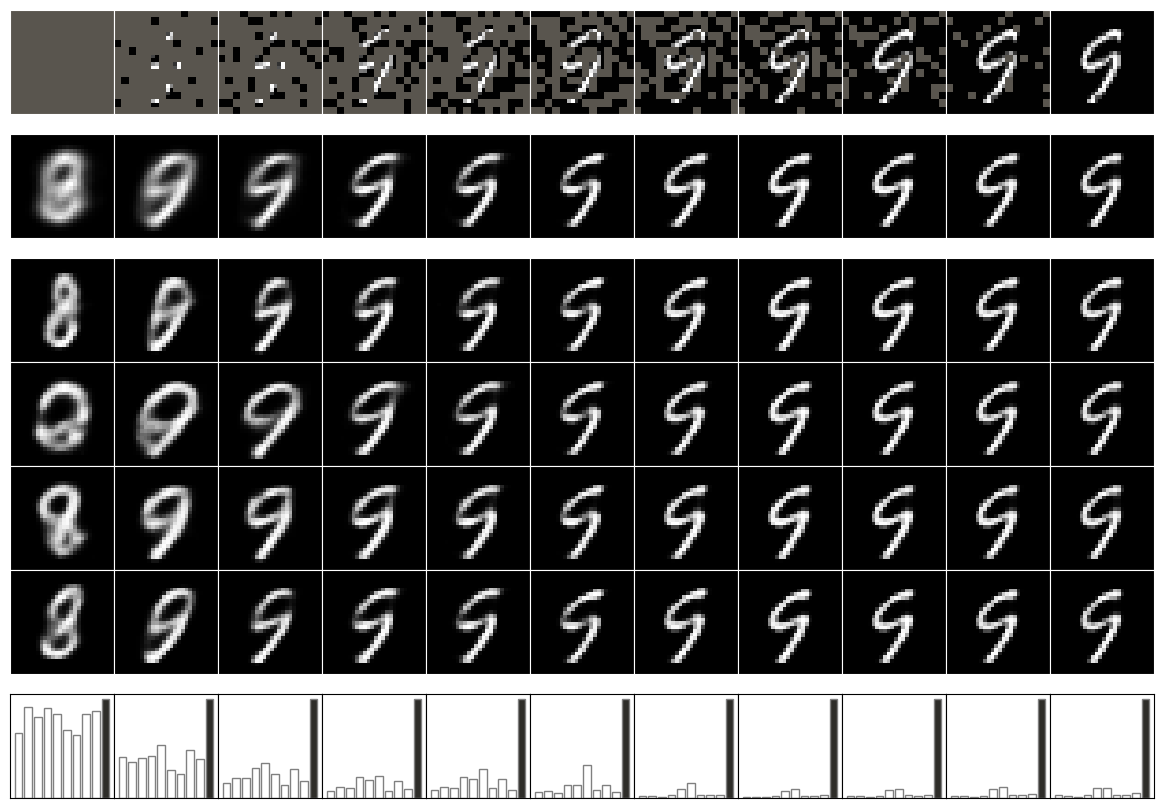
\includegraphics{figures/ivae/mnist/mnist-cvae-2.png}};
            
             \coordinate (left)  at ($(img.north west)!0.01!(img.north east)$);
            \coordinate (right) at ($(img.north west)!0.99!(img.north east)$);

            \foreach \i in {0,...,10} {
                \node[anchor=south] at ($(left)!{(\i + 0.5)/11}!(right)$) {{\fontsize{32}{36}\selectfont $\the\numexpr\i*10\relax\%$}};
            }

            \node[anchor=south] at ($(img.north)+(0,2.5)$) {{\fontsize{42}{48}\selectfont CVAE}};

            \node[anchor=east] at ($(img.north west)+(0,-2.2)$) {{\fontsize{32}{36}\selectfont observations}};
            \node[anchor=east] at ($(img.north west)+(0,-6.5)$) {{\fontsize{32}{36}\selectfont belief mean}};
            \node[anchor=east] at ($(img.north west)+(0,-10.8)$) {{\fontsize{32}{36}\selectfont state samples}};
            \node[anchor=east] at ($(img.south west)+(0,2.2)$) {{\fontsize{32}{36}\selectfont classification}};
            
        \end{tikzpicture}
    }

    \vspace*{5mm} % blank lines above and below are important

    \caption{MNIST example observations over time for the $\mathcal{I}$-VAE and CVAE models.}
    \label{fig:mnist_ivae_images1}
\end{figure}


\begin{figure}[p]
    \hspace*{5.5mm}
    \resizebox{0.8\linewidth}{!}{
        \begin{tikzpicture}
            \node[inner sep=0] (img) at (0,0) {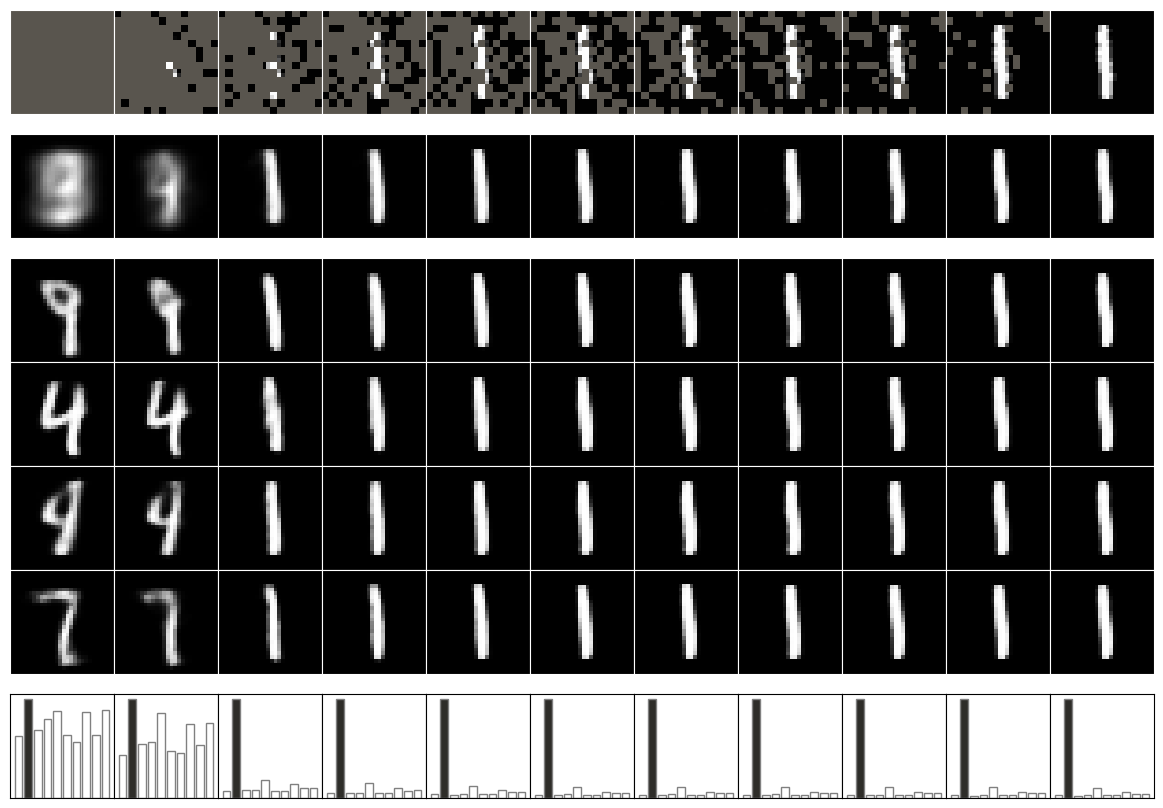
\includegraphics{figures/ivae/mnist/mnist-ivae-1.png}};
            
             \coordinate (left)  at ($(img.north west)!0.01!(img.north east)$);
            \coordinate (right) at ($(img.north west)!0.99!(img.north east)$);

            \foreach \i in {0,...,10} {
                \node[anchor=south] at ($(left)!{(\i + 0.5)/11}!(right)$) {{\fontsize{32}{36}\selectfont $\the\numexpr\i*10\relax\%$}};
            }

            \node[anchor=south] at ($(img.north)+(0,2.5)$) {{\fontsize{42}{48}\selectfont $\mathcal{I}$-VAE}};

            \node[anchor=east] at ($(img.north west)+(0,-2.2)$) {{\fontsize{32}{36}\selectfont observations}};
            \node[anchor=east] at ($(img.north west)+(0,-6.5)$) {{\fontsize{32}{36}\selectfont belief mean}};
            \node[anchor=east] at ($(img.north west)+(0,-10.8)$) {{\fontsize{32}{36}\selectfont state samples}};
            \node[anchor=east] at ($(img.south west)+(0,2.2)$) {{\fontsize{32}{36}\selectfont classification}};
            
        \end{tikzpicture}
    }

    \vspace*{15mm} % blank lines above and below are important
    
    \hspace*{5.5mm}
    \resizebox{0.8\linewidth}{!}{
        \begin{tikzpicture}
            \node[inner sep=0] (img) at (0,0) {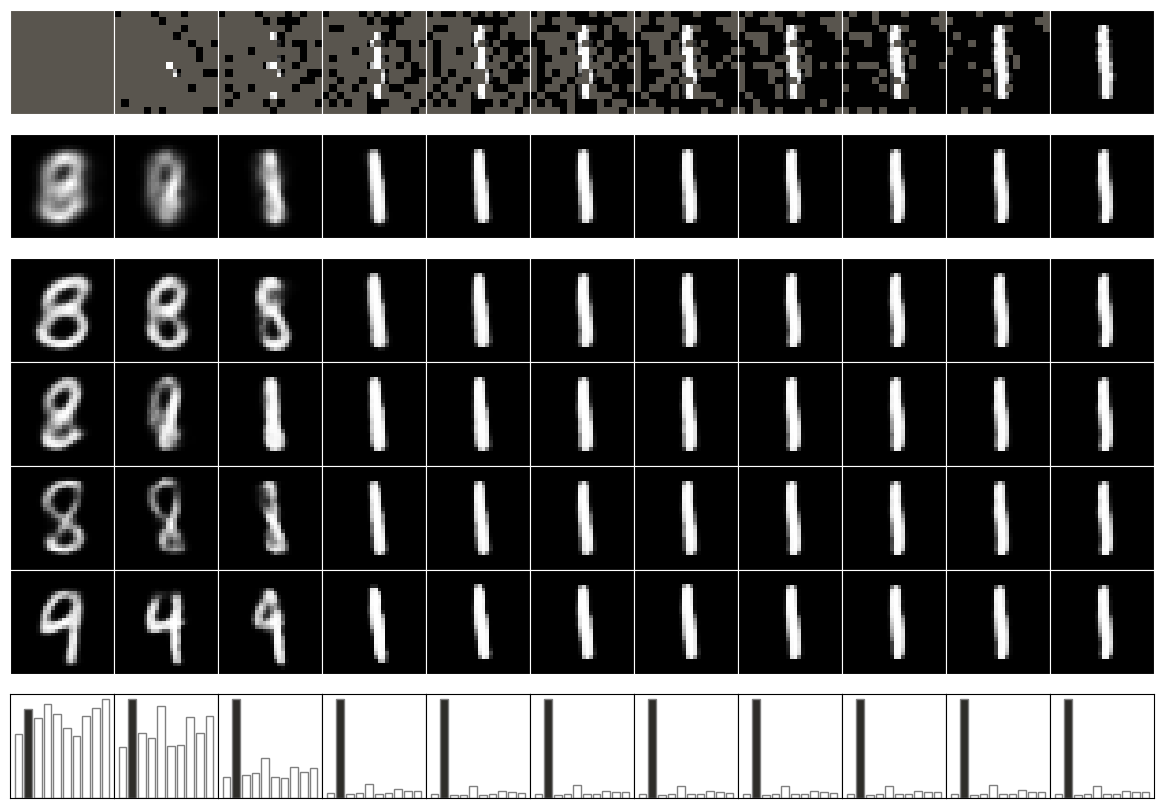
\includegraphics{figures/ivae/mnist/mnist-cvae-1.png}};
            
             \coordinate (left)  at ($(img.north west)!0.01!(img.north east)$);
            \coordinate (right) at ($(img.north west)!0.99!(img.north east)$);

            \foreach \i in {0,...,10} {
                \node[anchor=south] at ($(left)!{(\i + 0.5)/11}!(right)$) {{\fontsize{32}{36}\selectfont $\the\numexpr\i*10\relax\%$}};
            }

            \node[anchor=south] at ($(img.north)+(0,2.5)$) {{\fontsize{42}{48}\selectfont CVAE}};

            \node[anchor=east] at ($(img.north west)+(0,-2.2)$) {{\fontsize{32}{36}\selectfont observations}};
            \node[anchor=east] at ($(img.north west)+(0,-6.5)$) {{\fontsize{32}{36}\selectfont belief mean}};
            \node[anchor=east] at ($(img.north west)+(0,-10.8)$) {{\fontsize{32}{36}\selectfont state samples}};
            \node[anchor=east] at ($(img.south west)+(0,2.2)$) {{\fontsize{32}{36}\selectfont classification}};
            
        \end{tikzpicture}
    }

    \vspace*{5mm} % blank lines above and below are important

    \caption{Additional MNIST observations over time for the $\mathcal{I}$-VAE and CVAE models.}
    \label{fig:mnist_ivae_images2}
\end{figure}


\begin{figure}[t]
    \centering
    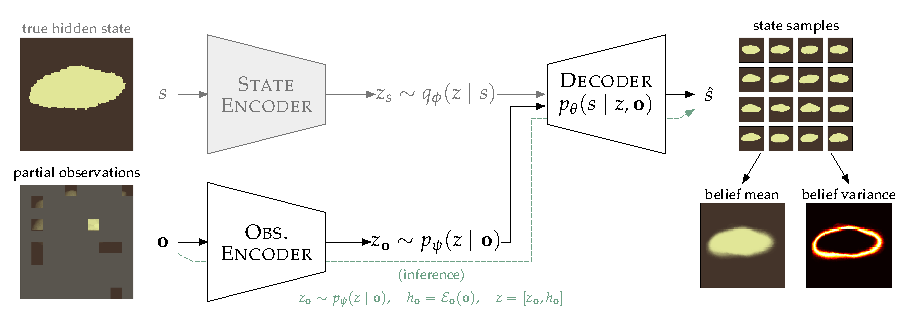
\includegraphics[width=\linewidth]{diagrams/ivae/muon-ivae-process.pdf}
    \caption{Muon observation inversion process using an $\mathcal{I}$-VAE with $10$ observations.}
    \label{fig:muon_ivae_process}
\end{figure}


\subsection{Indirect Observation Problem: Muon Tomography}
In the previous section, we showed how the $\mathcal{I}$-VAE model operates when treating pixel observations as a state mask.
In more realistic geological problems, different measurement sources, such as seismic imaging \cite{deng2022openfwi} or muon tomography \cite{schultz2007statistical,lechmann2021muon} (shown in \cref{fig:muon_ivae_process}), are used to infer the unknown state of the subsurface.
Statistical models of the subsurface are particularly useful as they capture the uncertainty in what's underground \cite{kaipio2006statistical}.

In the field of mineral exploration \cite{haldar2018mineral}, typical strategies consist of drilling or placing sensors in an exhaustive grid to collect subsurface information.
More recently, \textcite{mern2021improved} framed the mineral exploration problem as a POMDP and used state-of-the-art POMDP solvers to intelligently select where to drill, avoiding standard grid-based policies.
\textcite{mern2021improved} treated drill actions as observing borehole data to collect subsurface information.
Mineral exploration is a multi-objective problem: we want to maximize information gain while simultaneously minimizing the overall cost (e.g., minimizing the number of drills).
The ultimate objective of the mineral exploration problem is to make a \texttt{go}/\texttt{no-go} decision to \texttt{mine} or \texttt{abandon} based on some economic value of the subsurface intrusion (e.g., the mass of a subsurface ore body being worth the cost to extract).
The problem can be framed as an information gathering EMDP where the true state does not transition. 

\subsubsection{Sequential Information Gathering using Batched Belief-State Planning}

Crucial to the success of the POMDP solvers is the efficacy of the belief updater.
\textcite{mern2021improved} used a particle filter given a known observation model $O(o \mid a, s')$.
In our work, we study the case where the observation model is not known (or difficult to compute), the observations come from muon tomography projected to 2D, and drill actions place a row of $9$ passive muon sensors into the subsurface, as shown in 3D in \cref{fig:muon_intrusion_diagram}.
The muon tomography EMDP receives a penalty for every drill action executed, a reward proportional to the difference in the extracted intrusion mass compared to an economic threshold if the \texttt{go} action is taken, and zero reward in the case of a \texttt{no-go} decision.


\begin{figure}[t!]
    \captionsetup{font={small}}
    \centering
    \begin{subfigure}[t]{0.32\linewidth}
        \centering
        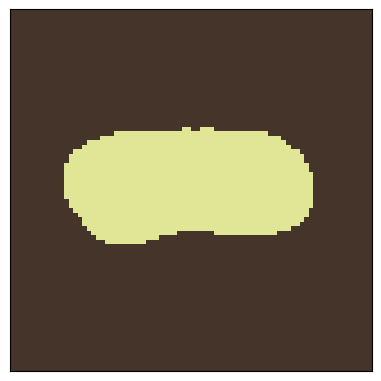
\includegraphics[width=0.9\linewidth]{figures/ivae/muon/muon-obs-state.png}
        \caption{Example input muon state.}
        \label{fig:muon_obs_state}
    \end{subfigure}
    \hfill
    \begin{subfigure}[t]{0.32\linewidth}
        \centering
        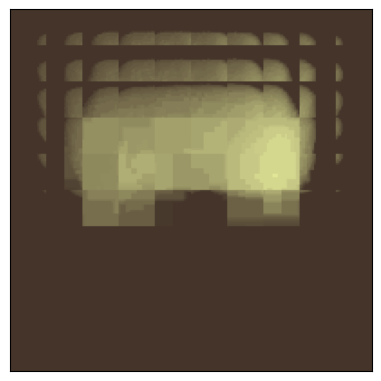
\includegraphics[width=0.9\linewidth]{figures/ivae/muon/muon-obs-simulated.png}
        \caption{Physics-based muon simulation.}
        \label{fig:muon_obs_simulated}
    \end{subfigure}
    \hfill
    \begin{subfigure}[t]{0.32\linewidth}
        \centering
        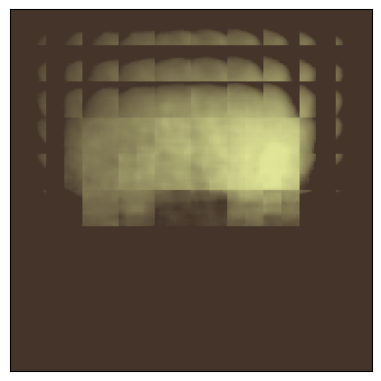
\includegraphics[width=0.9\linewidth]{figures/ivae/muon/muon-obs-surrogate.png}
        \caption{U-Net observation surrogate.}
        \label{fig:muon_obs_surrogate}
    \end{subfigure}
    \caption{Muon density U-Net surrogate model compared to the physics-based simulator.}
    \label{fig:muon_obs_model}
\end{figure}


\begin{figure}[b!]
    \captionsetup{font={small}}
    \centering
    \begin{subfigure}[t]{0.64\linewidth}
        \centering
        \resizebox{\linewidth}{!}{%
        \begin{tikzpicture}
            \node[yshift=15mm] {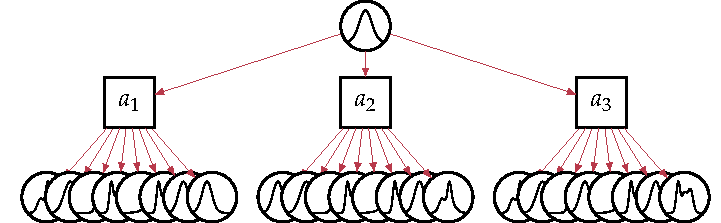
\includegraphics[width=\linewidth]{diagrams/ivae/onestep-lookahead-bmdp.pdf}};
            \node[] {\phantom{---}};
        \end{tikzpicture}}
        \caption{Belief-state MDP one-step lookahead over $3$ actions.}
        \label{fig:osl_bmdp}
    \end{subfigure}
    \hfill
    \begin{subfigure}[t]{0.32\linewidth}
        \centering
        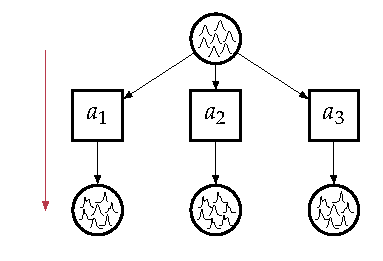
\includegraphics[width=\linewidth]{diagrams/ivae/onestep-lookahead-bbmdp.pdf}
        \caption{\textbf{BB}-MDP one-step lookahead.}
        \label{fig:osl_bbmdp}
    \end{subfigure}
    \caption{Indicating number of belief transition calls in red for BDMPs vs. \textbf{BB}-MDPs.}
    \label{fig:onestep_lookahead}
\end{figure}


Introduced in \cref{ch:bbmdp}, we convert the mineral exploration with muon tomography EMDP (termed \textit{muon-based intrusion discovery}) into its batched equivalent.
Aside from the observation function (which we cover next), the $\mathcal{I}$-VAE belief updater is designed to be parallel and, trivially, there are no state-transition dynamics.
As for the forward observation function, we trained a simple U-Net \cite{ronneberger2015unet} as a surrogate observation model (\cref{fig:muon_obs_model}) using data from a physics-based muon density simulator.
Therefore, we can directly convert the muon-based intrusion discovery problem into a \textbf{BB}-MDP.
Using this formulation, along with the neural network surrogates, we can sample $m$ state particles and evaluate all $100$ actions (corresponding to muon sensor drill locations) in one forward pass to the U-Net observation surrogate and one forward pass to the $\mathcal{I}$-VAE belief updater as a batch, shown compared to the standard belief-state MDP (BMDP) in \cref{fig:onestep_lookahead}.


\paragraph{Information-based heuristic policy.}
To test the performance of the $\mathcal{I}$-VAE belief updater in the batched planning setting, we use an information-based heuristic policy to maximize the expected Bayesian information gain.
The heuristic policy, shown in \cref{eq:muon_heuristic}, will pick drill locations $a \in \mathcal{A}$ over the $10 \times 10$ drilling sites that maximize expected information:
\begin{equation}
    \mathcal{H}(b) - \mathbb{E}_i\big[\mathcal{H}(b'_i)\big] \approx \mathbb{E}_i\left[ \sum_{s \in b'_i} b'_i(s)\log b'_i(s) \right] - \sum_{s \in b} b(s)\log b(s) \label{eq:expected_entropy_reduction}
\end{equation}
where $b'_i \in \mathbf{b}'$ and $\mathbf{b}' \sim \mathbf{T}_b(\cdot \mid \mathbf{b}, a)$ is an $m$-sized batch of beliefs, each with $k$ state particles.
In our experiments, we use $m = 3$ beliefs in the batch and $k=100$ state samples per belief.
We show that picking the action that maximizes the expected entropy reduction is equivalent to maximizing the expected KL-divergence objective (relating to the \textit{efficacy of information} (EOI) \cite{caers2022efficacy}).

\begin{theorem}[Equivalence of expected entropy reduction and expected KL-divergence]\label{thm:entropy_kl_equiv}
Let $b$ be a prior belief over the continuous state space $\mathcal{S}$.
Suppose we draw $m$ posterior beliefs $[b'_1, \ldots, b'_m] = \mathbf{b}'$ by sampling $b'_i \sim T_b(\cdot \mid b, a, o_i)$ following \cref{eq:tbb1,eq:tbb2,eq:tbb3,eq:tbb4}, then the expected reduction in entropy is equivalent to the expected KL-divergence between $\mathbf{b}'$ and $b$, namely:
\begin{equation}
    \mathcal{H}(b) - \mathbb{E}_i\big[\mathcal{H}(b'_i)\big] = \mathbb{E}_i \big[ \operatorname{KL}(b'_i \,\Vert\, b) \big] \quad \text{where} \quad b'_i \in \mathbf{b}' \label{eq:entropy_thm}
\end{equation}
This results in an optimal one-step information gathering policy that maximizes Bayesian information gain.
Subsequently, this can be computed using the Monte Carlo estimate:
\begin{equation}
    \mathcal{H}(b) - \mathbb{E}_i\big[\mathcal{H}(b'_i)\big] \approx \frac{1}{m} \sum_{i=1}^m \left( \sum_{s \in b'_i} b'_i(s) \log b'_i(s) \right) - \sum_{s \in b} b(s) \log b(s)    
\end{equation}
As $m \to \infty$ and the state particle count $k \to \infty$, this converges to the true expected KL-divergence:
\begin{equation}
    \mathbb{E}_i \big[ \operatorname{KL}(b'_i \,\Vert\, b) \big] = \lim_{\substack{m \to \infty \\ k \to \infty}} \left[ \frac{1}{m} \sum_{i=1}^m \left( \sum_{s_j}^k b'_i(s_j) \log b'_i(s_j) \right) - \sum_{s_j}^k b(s_j) \log b(s_j) \right]
\end{equation}
\end{theorem}

\begin{proof}
    We show that the expected entropy reduction of the belief is exactly the expected KL-divergence between each posterior and the prior, justifying the use of this measurement when selecting actions to maximize expected information gain.
    For each posterior belief $b'_i$, the KL-divergence can be expressed as:
    \begin{align}
        \operatorname{KL}(b'_i \,\Vert\, b) &= \int b'_i(s) \log b'_i(s) \diff s - \int b'_i(s) \log b(s) \diff s \\
            &= -\mathcal{H}(b'_i) - \int b'_i(s) \log b(s) \diff s
    \end{align}
    Rearranging and adding $\mathcal{H}(b)$ to both sides, we get:
    \begin{equation}
        \mathcal{H}(b) - \mathcal{H}(b'_i) = \operatorname{KL}(b'_i \,\Vert\, b) + \int b'_i(s) \log b(s) \diff s + \mathcal{H}(b)
    \end{equation}
    Because $b'_i$ is generated by first sampling $s \sim b$, followed by $s' \sim T(\cdot \mid s, a)$, $o \sim O(\cdot \mid a, s')$, and updated using $b' = \textsc{Update}(b, a, o)$, by the law of total expectation, we get:
    \begin{align}
        \mathbb{E}_i\left[ \int b'_i(s) \log b(s) \diff s \right] &= \operatorname*{\mathbb{E}}_{s \sim b} \Bigg[ \operatorname*{\mathbb{E}}_{(s',o \mid s)} \bigg[ \mathbb{E}_{b'_i} \Big[\log b(s)\Big] \bigg] \Bigg] \\
            &= \mathbb{E}_{s}\big[ \log b(s) \big] \\
            &= \int b(s) \log b(s) \diff s \\
            &= -\mathcal{H}(b)
    \end{align}
    Now using this result in the expanded definition of expected entropy reduction, we get:
    \begin{align}
        \mathcal{H}(b) - \mathbb{E}_i\big[\mathcal{H}(b'_i)\big] &= \mathbb{E}_i \left[ \mathcal{H}(b) - \mathcal{H}(b'_i) \right] \\
            &= \mathbb{E}_i \Bigg[ \operatorname{KL}(b'_i \,\Vert\, b) + \underbrace{\int b'_i(s) \log b(s) \diff s}_{-\mathcal{H}(b)} + \mathcal{H}(b) \Bigg] \\
            &= \mathbb{E}_i \big[ \operatorname{KL}(b'_i \,\Vert\, b) \big]
    \end{align}
    Therefore, we reach our desired equivalence of:
    \begin{equation}
        \mathcal{H}(b) - \mathbb{E}_i\big[\mathcal{H}(b'_i)\big] = \mathbb{E}_i \big[ \operatorname{KL}(b'_i \,\Vert\, b) \big]
    \end{equation}
\end{proof}

Using the results from \cref{thm:entropy_kl_equiv}, the information-based heuristic policy will select actions that maximize the information gain, then make a final decision based off the probability that the economic intrusion volume is above some risk threshold $1 - \Delta$.
The heuristic policy is defined as:
\begin{equation}
    \pi_\text{heuristic}(b) = \begin{cases}
        \texttt{go} & \text{if } P(v > 0) > 1 - \Delta \\
        \texttt{no-go} & \text{if } P(v < 0) > 1 - \Delta \\
        \argmax\limits_{a \in \mathcal{A}} \mathcal{H}(b) - \mathbb{E}_i\big[\mathcal{H}(b'_i)\big] & \text{otherwise}
    \end{cases} \label{eq:muon_heuristic}
\end{equation}
where the distribution over intrusion volume $v$ is computed over the belief $b$ and standardized so that the nominal (prior) volume has zero mean.
When the standardized volume is above zero, this indicates the intrusion is economical to mine.
This way, if we randomly took \texttt{go}/\texttt{no-go} actions, we would make the correct decision $50\%$ of the time.
The parameter $\Delta$ controls the risk tolerance in the final \texttt{go}/\texttt{no-go} decision.
In the following experiments, we set $\Delta = 0.1$, resulting in making the final decision if the confidence in our estimated volume distribution is above $90\%$.
Other criterion, such as the upper-confidence bound (UCB$1$) algorithm \cite{auer2002finite} or Bayes-UCB \cite{kaufmann2012bayesian}, could be used instead.


\paragraph{Baseline policies.}
Along with the heuristic policy, we evaluate four other baseline policies.
The first two baseline policies select actions deterministically following sweeping grid-like patterns.
Starting from the top-left origin of the $10 \times 10$ action space, the \textit{horizontal grid} policy selects actions in a right-to-left, then left-to-right sweeping pattern.
Similarly, the \textit{vertical grid} policy selects actions in a downward, then upward pattern; mimicking conventional drilling strategies \cite{haldar2018mineral}.
We also baseline against a \textit{random} policy that will randomly select actions uniformly over the action space.
Finally, given privileged information about the true state under test, we test against an \textit{oracle} that selects the action that minimizes the error between the mean posterior belief and the true state (with access to truth):
\begin{equation}
    \pi_\text{oracle}(b) = \begin{cases}
        \texttt{go} & \text{if } P(v > 0) > 1 - \Delta \\
        \texttt{no-go} & \text{if } P(v < 0) > 1 - \Delta \\
        \argmin\limits_{a \in \mathcal{A}} \Big|\mathbb{E}[b'] - s_\text{true}\Big| & \text{otherwise}
    \end{cases}\label{eq:muon_oracle}
\end{equation}
The oracle policy determines the best performance that each belief updater could achieve.
We compare the $\mathcal{I}$-VAE with and without TCL fine-tuning, the CVAE model, and a particle filter with reinvigoration where the estimated observation likelihood measures how close each observation is to a sampled state from the belief, proportional to the mean-squared error between the observation generated from the sampled state and the environment observation.


\begin{table*}[b!]
    \centering
    \begin{threeparttable}
        \begin{tabular}{@{}lrrrrr@{}}
            \toprule
            \multirow{2}{*}{Method} & \multicolumn{5}{c}{Conditional log-likelihood (CLL)} \\
            \cmidrule{2-6}
            & $0$ & $25$ & $50$ & $75$ & $100$ \\
            \midrule
            CVAE                        &  $\mathBF{-563.41}$      &  $-213.98$  &  $-169.42$  &  $-148.90$  &  $-141.17$  \\
            $\mathcal{I}$-VAE (no TCL)  &  $-692.58$  &  $-173.47$  &  $-155.47$  &  $-144.20$  &  $-127.79$  \\
            $\mathcal{I}$-VAE           &  $-657.39$  &  $\mathBF{-159.04}$  &  $\mathBF{-147.93}$  &  $\mathBF{-136.54}$  &  $\mathBF{-125.45}$  \\
            \bottomrule
        \end{tabular}
    \end{threeparttable}
    \caption{Muon problem: CLLs given different numbers of observations.}
    \label{tab:clls_muon}
\end{table*}


\paragraph{Planning and estimation metrics.}
We use several metrics to compare how well the $\mathcal{I}$-VAE estimates the conditional likelihood $p(s \mid \mathbf{o})$ and its performance during planning.
For estimation quality, we use the conditional log-likelihood defined in \cref{eq:cll}.
To evaluate the planning performance using the heuristic and baseline policies, we measure the accuracy in the final \texttt{go}/\texttt{no-go} decision (where \texttt{go} should be executed if the economic volume of a test intrusion is above zero), and we measure how many actions it took to reach the final decision.
Finally, we measure the error in the belief compared to the true test state over different number of actions/observations.

\subsubsection{Muon-Based Intrusion Discovery Results and Analysis}

\Cref{tab:clls_muon} and \cref{fig:clls_muon} show the estimation performance of the neural network belief surrogates.
When selecting drill actions, each surrogate uses the information-based heuristic policy \textit{without} making a final decision (to ultimately evaluate the performance over all drill actions).
Evident in our experiments, we see that the $\mathcal{I}$-VAE belief updater achieves better estimation qualities when compared to the CVAE and the $\mathcal{I}$-VAE without TCL.
Unlike the MNIST example, in the muon tomography case, the initial belief (i.e., conditioned on no observations) is more diffuse, resulting in worse early estimation performance.


\begin{figure}[t!]
    \centering
    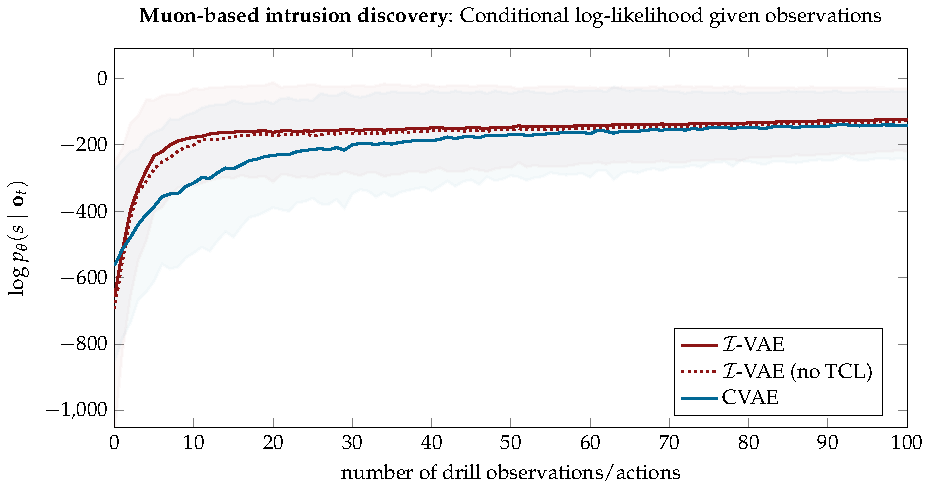
\includegraphics[width=0.825\linewidth]{figures/ivae/muon/cll-muon.pdf}
    \caption{Conditional log-likelihood for the muon problem using the heuristic policy.}
    \label{fig:clls_muon}
\end{figure}


\begin{table*}[b!]
    \centering
    \begin{threeparttable}
        \begin{adjustbox}{max width=\textwidth}
        \begin{tabular}{@{}lrrrr|r@{}}
            \toprule
            \multirow{4}{*}{Method} & \textsc{Grid (horiz.)} & \textsc{Grid (vert.)} & \textsc{Random} & \textsc{Heuristic} & \textsc{Oracle} \\
            \cmidrule{2-6}
            & Accuracy $\uparrow$ & Accuracy $\uparrow$ & Accuracy $\uparrow$ & Accuracy $\uparrow$ & Accuracy $\uparrow$ \\
            & \texttt{\#} Actions $\downarrow$ & \texttt{\#} Actions $\downarrow$ & \texttt{\#} Actions $\downarrow$ & \texttt{\#} Actions $\downarrow$ & \texttt{\#} Actions $\downarrow$ \\
            \midrule
            \multirow{2}{*}{Particle filter\tnote{$\dagger$}}  &  $0.75  \pm  0.03$   &  $0.65  \pm  0.03$   &  $0.67  \pm  0.03$   &  ---   &  ---  \\
                                                         &  $89.00  \pm  1.03$  &  $76.17  \pm  1.13$  &  $76.52  \pm  1.02$  &  ---   &  ---  \\
            \arrayrulecolor{white}\midrule
            \multirow{2}{*}{CVAE}                        &  $0.92  \pm  0.02$            &  $0.925  \pm  0.02$  &  $0.925  \pm  0.02$  &  $0.925  \pm  0.02$  &  $0.935  \pm  0.02$  \\
                                                         &  $\mathBF{27.38  \pm  1.79}$  &  $35.40  \pm  1.80$  &  $24.36  \pm  2.05$  &  $20.65  \pm  1.84$  &  $21.86  \pm  1.85$  \\
            \arrayrulecolor{white}\midrule
            \multirow{2}{*}{$\mathcal{I}$-VAE (no TCL)}  &  $\mathBF{0.925  \pm  0.02}$  &  $\mathBF{0.955  \pm  0.01}$  &  $0.935  \pm  0.02$  &  $0.95  \pm  0.02$  &  $0.975  \pm  0.01$  \\
                                                         &  $28.85  \pm  1.24$           &  $34.02  \pm  1.53$           &  $18.78  \pm  1.47$  &  $7.46  \pm  0.97$  &  $9.62   \pm  1.45$  \\
            \arrayrulecolor{white}\midrule
            \multirow{2}{*}{$\mathcal{I}$-VAE}           &  $\mathBF{0.925  \pm  0.02}$  &  $\mathBF{0.955  \pm  0.01}$  &  $\mathBF{0.95   \pm  0.02}$  &  $\mathBF{0.96  \pm  0.01}$  &  $\mathBF{0.99  \pm  0.01}$  \\
                                                         &  $28.45  \pm  1.31$           &  $\mathBF{31.11  \pm  1.39}$  &  $\mathBF{14.53  \pm  0.90}$  &  $\mathBF{6.88  \pm  0.85}$  &  $\mathBF{8.15  \pm  1.22}$  \\
            \arrayrulecolor{black} % revert
            \bottomrule
        \end{tabular}
        \end{adjustbox}
        \begin{scriptsize}
            \begin{tablenotes}
                \item[$\dagger$] {Heuristic and oracle results were omitted because the particle filter does not inherently support parallelism.}
            \end{tablenotes}
        \end{scriptsize}
    \end{threeparttable}
    \caption{Muon problem: Planning metrics comparing various policies and belief updaters.}
    \label{tab:muon_results}
\end{table*}


\begin{figure}[t!]
    \centering
    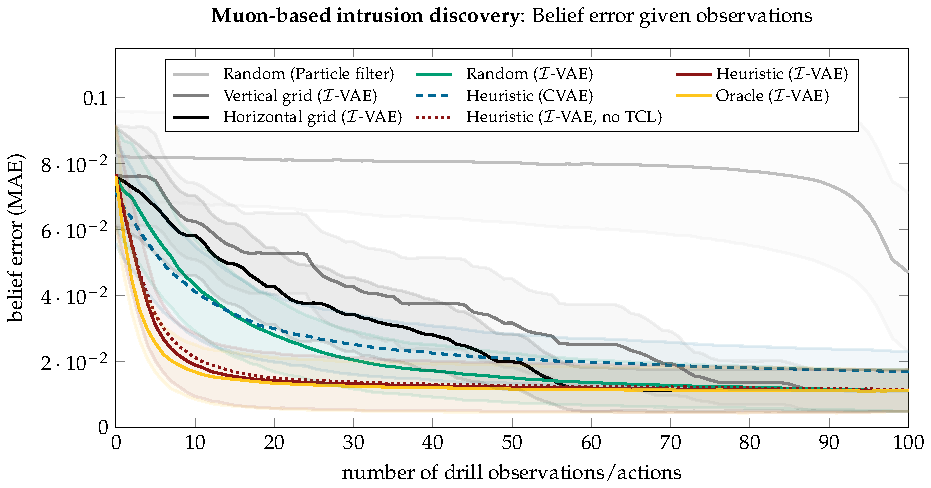
\includegraphics[width=0.825\linewidth]{figures/ivae/muon/muon-belief-error.pdf}
    \caption{Belief error relative to holdout test states for different policies and updaters.}
    \label{fig:belief_error_muon}
\end{figure}


\begin{figure}[b!]
    \captionsetup{font={small}}
    \centering
    \begin{subfigure}[t]{0.4715\linewidth}
        \centering
        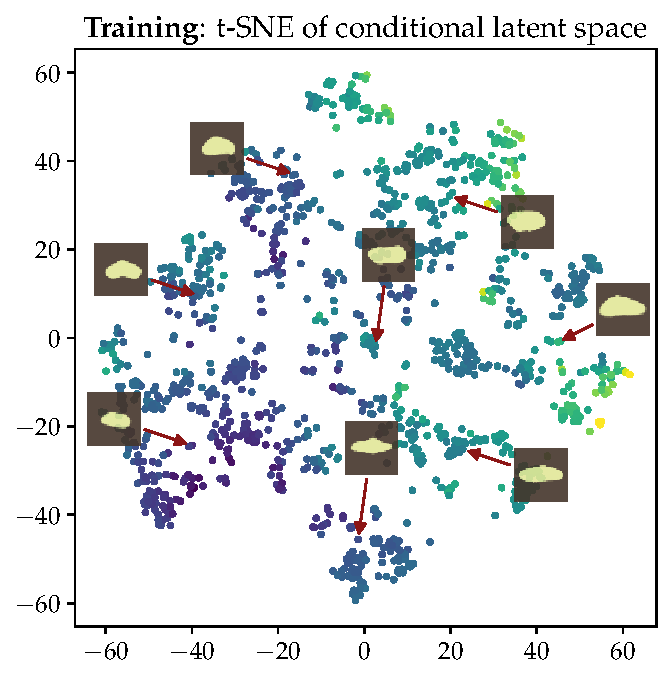
\includegraphics[width=0.925\linewidth]{figures/ivae/muon/tsne_muon_training.pdf}
        \caption{Conditional latent space ($1800$ training data).}
        \label{fig:tsne_muon_training}
    \end{subfigure}
    \hfill
    \begin{subfigure}[t]{0.48\linewidth}
        \centering
        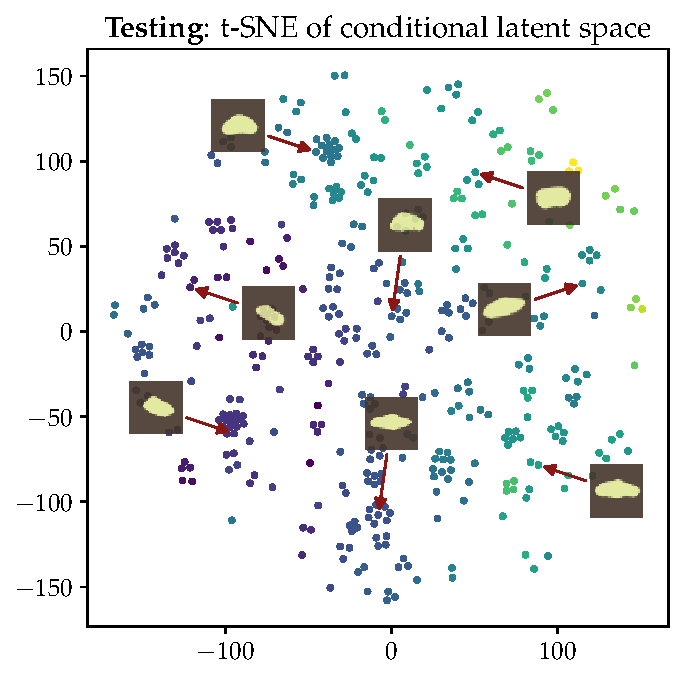
\includegraphics[width=0.925\linewidth]{figures/ivae/muon/tsne_muon_testing.pdf}
        \caption{Conditional latent space ($200$ testing data).}
        \label{fig:tsne_muon_testing}
    \end{subfigure}
    \caption{Visualizing the conditional latent space $p_\psi(z \mid \mathbf{o})$, colored by intrusion volume.}
    \label{fig:tsne}
\end{figure}


Regarding planning performance, \cref{tab:muon_results} indicates that the $\mathcal{I}$-VAE model produces the highest accuracy in the fewest number of actions.
We also highlight that the additional TCL fine-tuning step improves the base model.
Comparing the belief updating results in \cref{tab:muon_results} to their respective oracle column shows the theoretically one-step optimal performance achievable by each method.
This is also evident when looking at the belief error in \cref{fig:belief_error_muon} and comparing the $\mathcal{I}$-VAE heuristic to the $\mathcal{I}$-VAE oracle, which shows that the information-based heuristic is approximately optimal.
It is also clear that the particle filter performs poorly on this problem as it suffers from particle depletion (i.e., the belief collapses).
This is because the particle filter initially samples $k = 900$ state particles from the prior training data to represent its belief---using the same training states as the CVAE and $\mathcal{I}$-VAE models, given those states are the only examples each model has access to.
Sampling the finite state particles results in the inability of the particle filter to generate new states that are consistent with the observations but may not directly exist in the finite prior data.
This highlights the usefulness of learning generative models to act as approximate belief updaters.

Because the $\mathcal{I}$-VAE model explicitly learns parameters $\mu_\mathbf{o}$ and $\log \sigma^2_\mathbf{o}$ for the conditional prior $p_\psi(z \mid \mathbf{o})$, instead of a unit Gaussian, we can easily visualize the latent space using the t-SNE dimensionality reduction technique \cite{platzer2013visualization}.
Visualized in \cref{fig:tsne}, we can inspect the latent space and qualitatively determine that it learns to cluster observations based on the economic volume of the reconstructed states (shown in the colors).
The inlet plots show the average state reconstruction over $100$ samples.

Finally, \cref{fig:muon_trajectories} illustrates three example planning trajectories showing the belief mean over $100$ sampled states (where drill action locations are marked in red) and we show the economic intrusion volume distribution.
Quantitatively, in each of these three cases, we see that the heuristic planner using the $\mathcal{I}$-VAE model converges close to the true intrusion volume.
Qualitatively, these examples illustrate that the $\mathcal{I}$-VAE model accurately constructs a belief that converges, in shape, to the true state.
The figure shows the mean belief and volume distributions after a fixed number of actions, as well as the final belief and volume distribution when all $100$ drill actions are taken, where the blue lines indicate the true intrusion volume and the dashed red lines indicate the estimated mean from the belief.


\begin{figure}[p!]
    \captionsetup{font={small}}
    \centering
    \begin{subfigure}[t]{\linewidth}
        \centering
        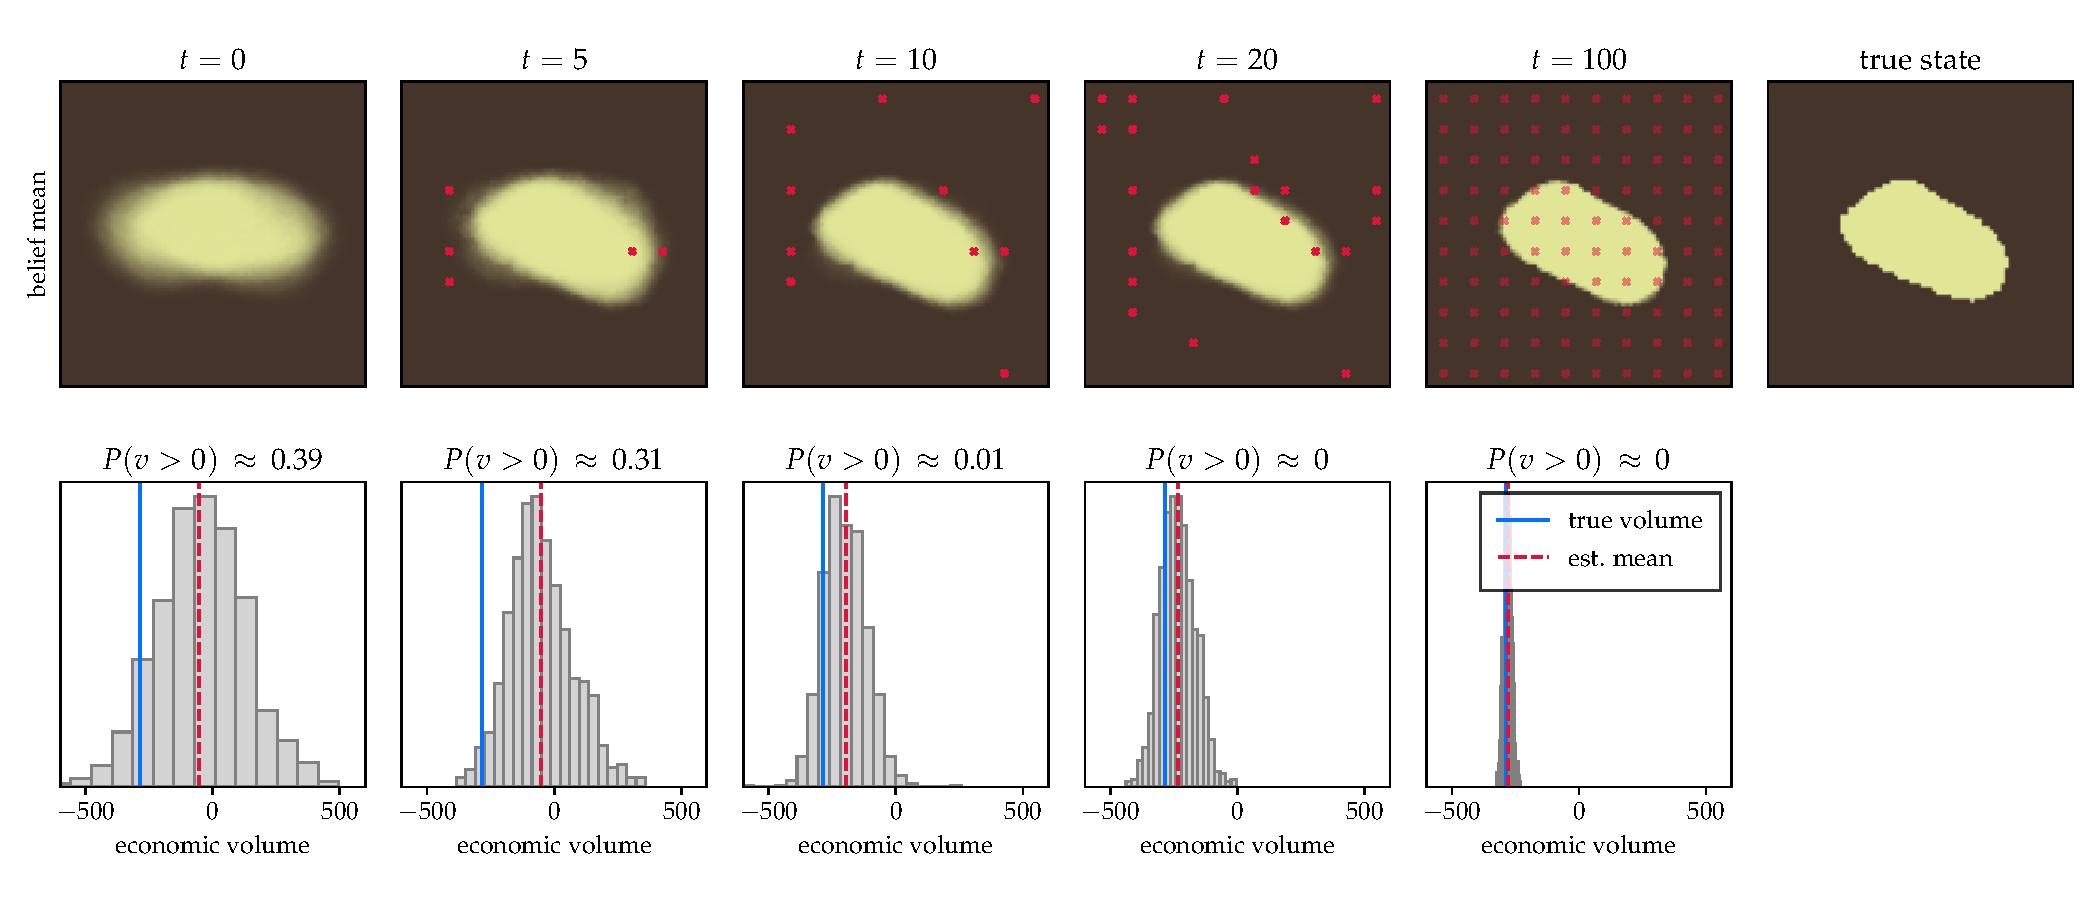
\includegraphics[width=0.92\linewidth]{figures/ivae/muon/muon_planning_59.pdf}
        \caption{Intrusion planning where the true volume is \textit{below} the economic threshold.}
        \label{fig:muon_planning_under}
    \end{subfigure}
    \begin{subfigure}[t]{\linewidth}
        \centering
        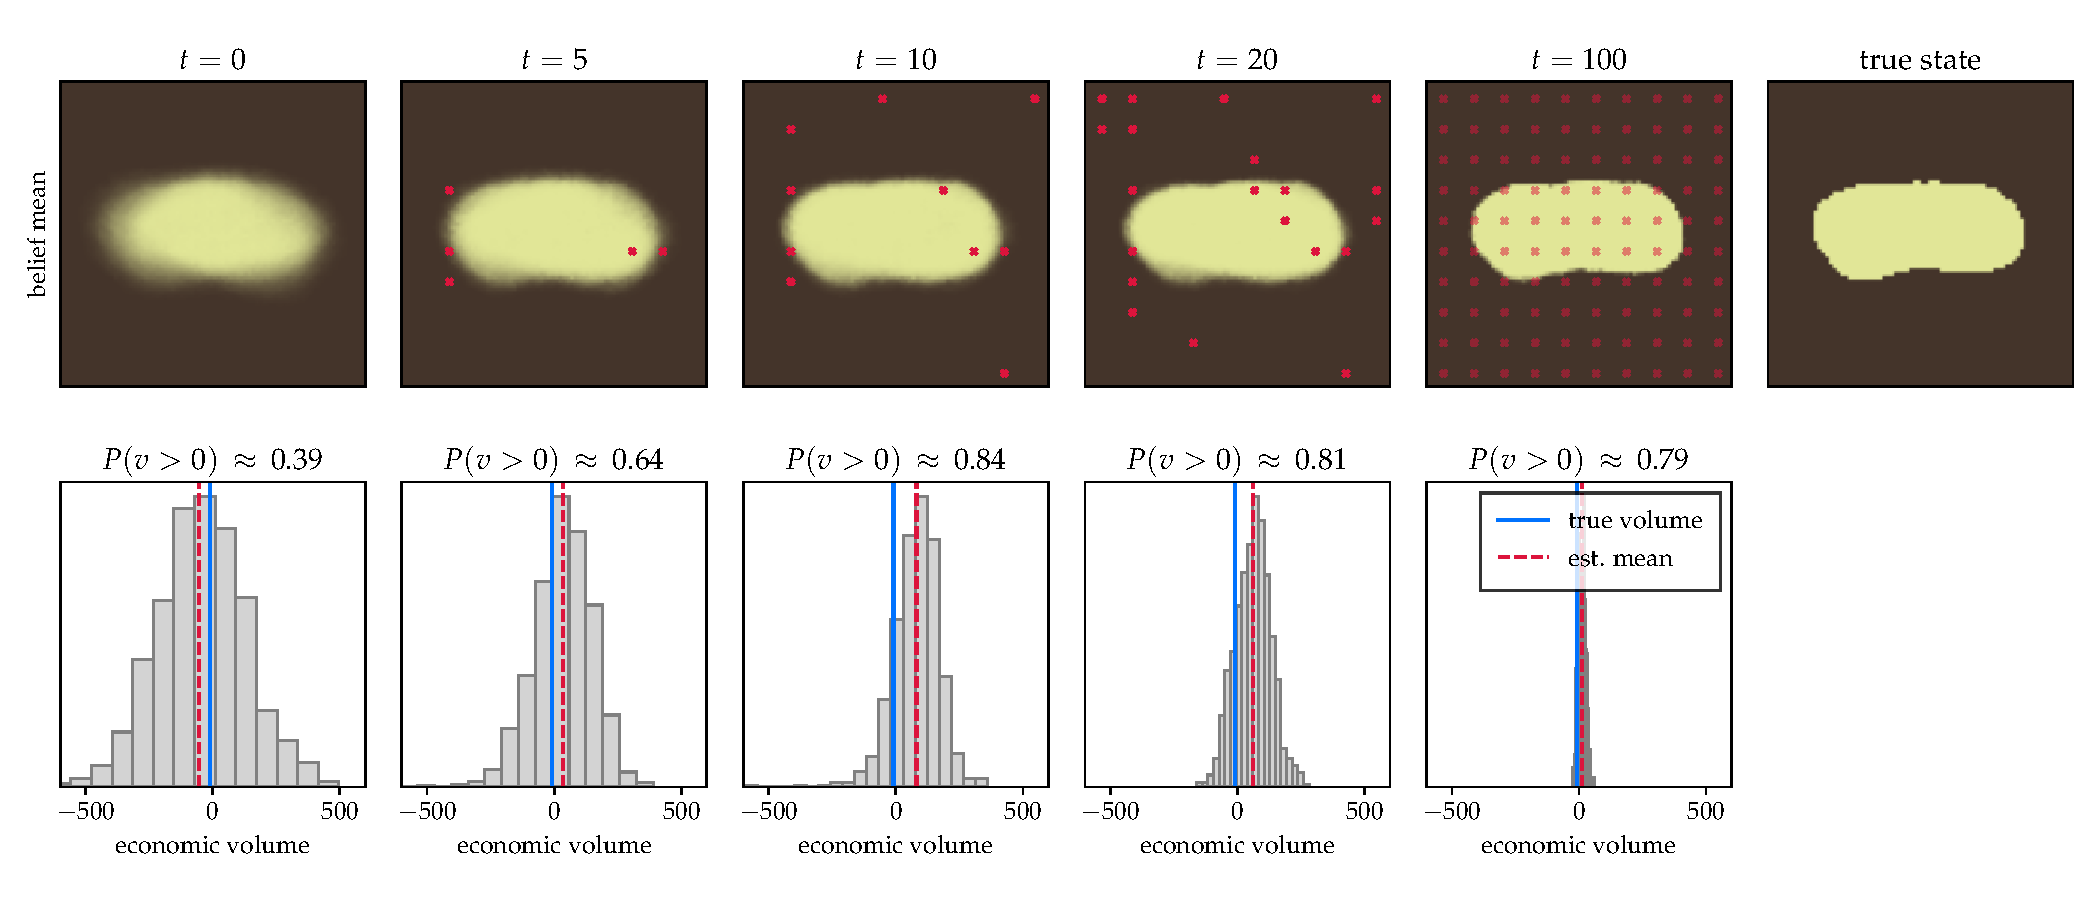
\includegraphics[width=0.92\linewidth]{figures/ivae/muon/muon_planning_2.pdf}
        \caption{Intrusion planning where the true volume is \textit{near} the economic threshold.}
        \label{fig:muon_planning_zero}
    \end{subfigure}
    \begin{subfigure}[t]{\linewidth}
        \centering
        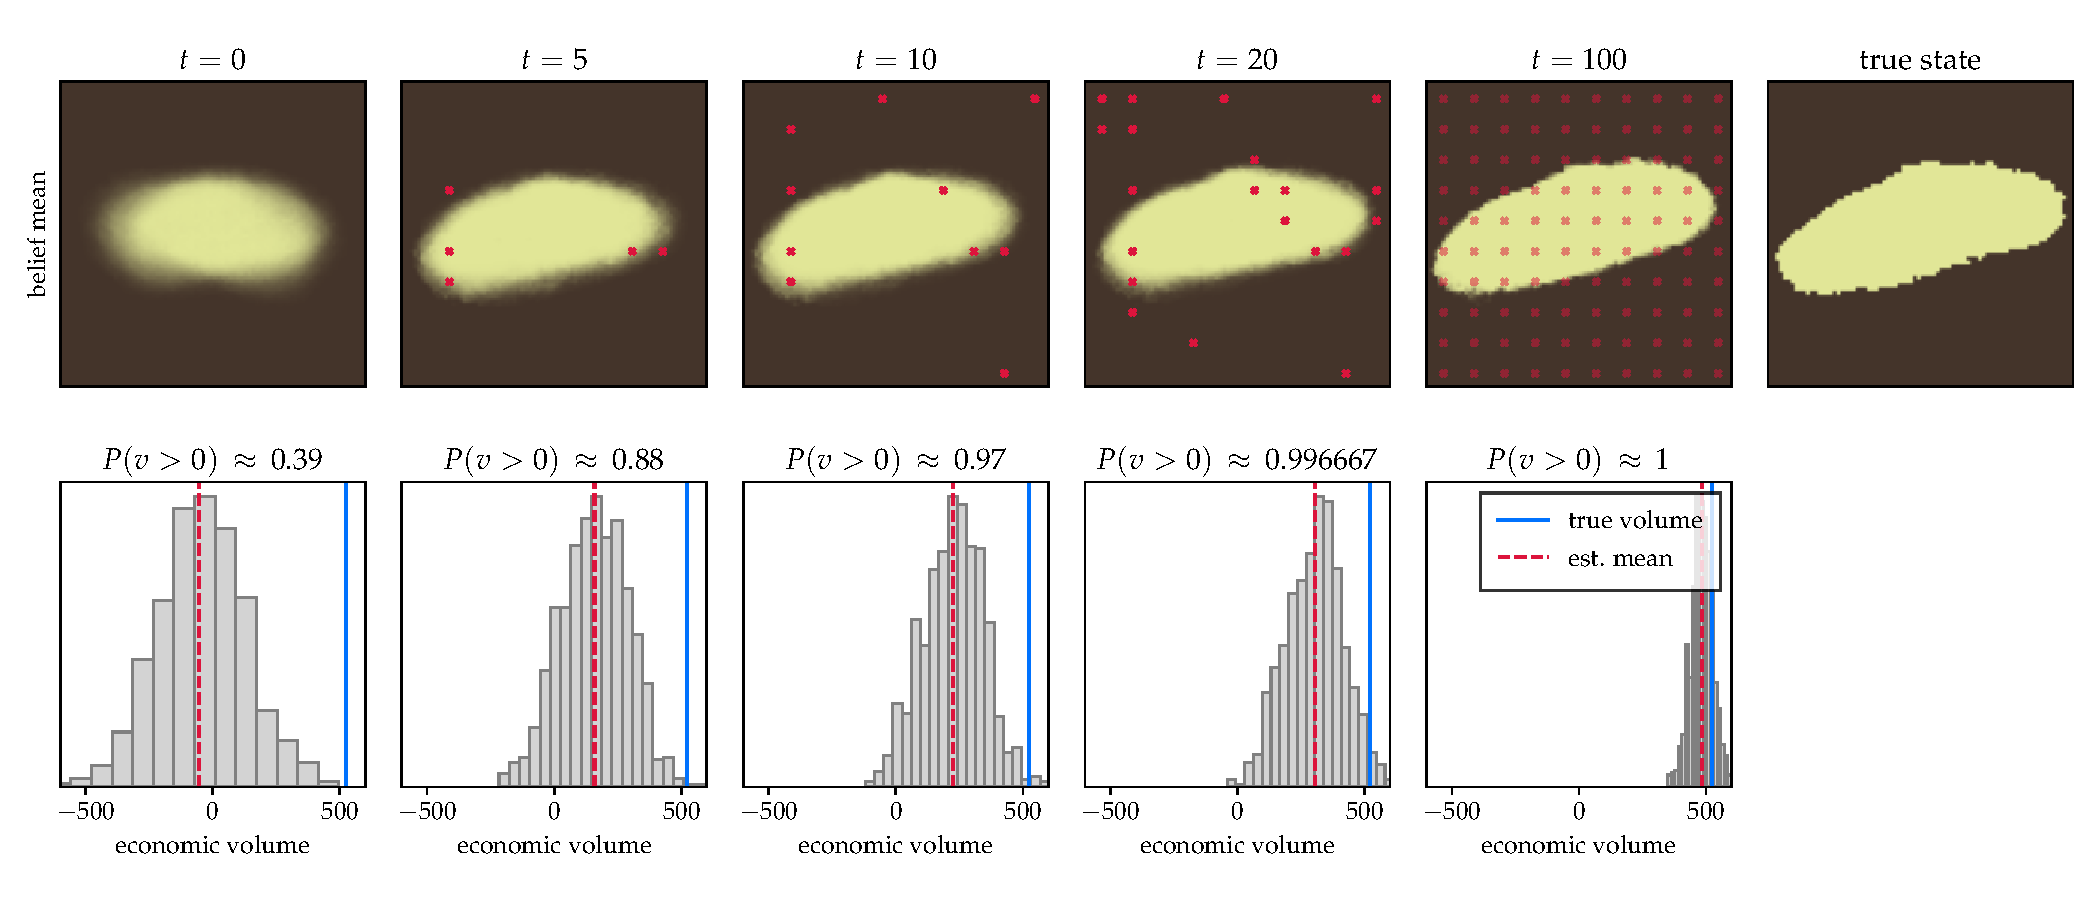
\includegraphics[width=0.92\linewidth]{figures/ivae/muon/muon_planning_82.pdf}
        \caption{Intrusion planning where the true volume is \textit{above} the economic threshold.}
        \label{fig:muon_planning_over}
    \end{subfigure}
    \caption{Beliefs for the muon-based intrusion discovery problem using the $\mathcal{I}$-VAE model.}
    \label{fig:muon_trajectories}
\end{figure}


\section{Conclusions}
In this chapter, we introduced a conditional deep generative model to approximate the belief update in an EMDP.
We framed the EMDP problem as its batched equivalent using the framework introduced in \cref{ch:bbmdp}.
To plan efficiently over batches, we introduced the \textit{inversion variational autoencoder} ($\mathcal{I}$-VAE) model that learns a latent distribution over states and a matching latent distribution over partial observations.
Given our sequential decision making setting, we further refine the model during a fine-tuning step to maximize the mutual information between latent variables along the same observation trajectories.
We showed that this model works well in cases where the observations are masked versions of the state and when the observations are indirectly related to the state through a forward model.
We demonstrated the model performance when used as a surrogate belief updater in a muon-based intrusion discovery problem, and showed that an information-based heuristic policy works well in this setting.
Insights from this work highlight that in problems with limited data, e.g., geological problems, using generative models allows for the creation of unseen states that are consistent with both the prior and the conditioning observations.
